\chapter{Algoritmo de Chu–Liu/Edmonds}

O algoritmo de Chu–Liu/Edmonds encontra uma r-arborescência de custo mínimo em um digrafo ponderado. A estratégia funciona de forma gulosa ao escolher, para cada vértice \(v\neq r\), o arco de entrada mais barato. No entanto, essa abordagem pode gerar ciclos dirigidos, incompatíveis com a estrutura de arborescência. O algoritmo resolve esse problema combinando normalização de custos, contração de ciclos em supervértices e expansão controlada para garantir otimalidade.

\section{O problema dos ciclos e a solução por contração}

Em uma r-arborescência, cada \(v\neq r\) deve ter exatamente um arco de entrada e \(r\) tem grau de entrada zero. Se escolhermos para cada vértice o arco mais barato que nele entra, podemos formar um ciclo dirigido \(C\) onde todos os vértices recebem seu único arco de dentro do próprio \(C\). Nesse caso, nenhum arco entraria em \(C\) a partir de \(V\setminus C\) (o corte \(\delta^-(C)\) ficaria vazio) e, como \(r\notin C\), não existiria caminho de \(r\) para os vértices de \(C\), contrariando a alcançabilidade exigida.

A Figura \ref{fig:chu-liu-cycle-micro} ilustra com um microexemplo: três vértices \(a,b,c\) (todos fora de \(r\)) onde o arco mais barato que entra em \(b\) vem de \(a\), o de \(c\) vem de \(b\) e o de \(a\) vem de \(c\), formando o ciclo \(a\to b\to c\to a\). Embora existam arcos de \(r\) para cada vértice, eles são mais caros e não são escolhidos pelo critério local, deixando os vértices "presos" no ciclo sem conexão com a raiz.

\begin{figure}[H]
    \centering
    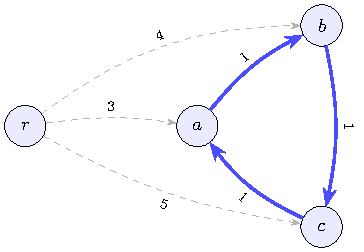
\includegraphics[width=0.9\linewidth]{figures/fig_chu_liu_cycle_micro.pdf}
    \caption{Ciclo gerado pelas escolhas locais "mais baratas por vértice". Os arcos grossos (custo 1) entram em \(a,b,c\) e formam \(a\to b\to c\to a\). Os arcos tracejados partindo de \(r\) existem, mas são mais caros e por isso não são escolhidos pelo critério local.}
    \label{fig:chu-liu-cycle-micro}
\end{figure}

A solução consiste em \emph{normalizar os custos por vértice}: para cada \(v\neq r\), subtraímos de todo arco que entra em \(v\) o menor custo entre os arcos que chegam a \(v\). Após esse ajuste (custos reduzidos), cada \(v\neq r\) passa a ter ao menos um arco de custo reduzido zero. Se os arcos de custo zero forem acíclicos, já temos a r-arborescência ótima. Se formarem um ciclo \(C\), \emph{contraímos} \(C\) em um \textbf{supervértice} \(x_C\), ajustamos os custos dos arcos externos e resolvemos recursivamente no grafo menor. Ao final, \emph{expandimos} as contrações removendo exatamente um arco interno de cada ciclo para manter grau de entrada 1 e aciclicidade global.

\subsection{Supervértices e contração de ciclos}

Dado um subconjunto \(C\subseteq V\) que forma um ciclo dirigido, a \emph{contração de \(C\)} substitui todos os vértices de \(C\) por um único vértice \(x_C\) — o supervértice. Todo arco com exatamente uma ponta em \(C\) passa a ser incidente a \(x_C\): arcos \((u,w)\) com \(u\notin C\), \(w\in C\) tornam-se \((u, x_C)\); arcos \((w,v)\) com \(w\in C\), \(v\notin C\) tornam-se \((x_C, v)\); e arcos com ambas as pontas em \(C\) são descartados.

Para preservar a comparação relativa dos custos, ajustamos os arcos que \emph{entram} em \(C\): para um arco \((u,w)\) com \(w\in C\), definimos \(c'(u,x_C) = c(u,w) - c(a_w)\), onde \(a_w\) é o arco mais barato que entra em \(w\). Essa normalização garante que decisões ótimas no grafo contraído podem ser traduzidas de volta na expansão.

\begin{figure}[H]\centering
    \begin{tikzpicture}[>=Stealth, node distance=1.4cm]
        % (a) Original
        \node at (-4.4,2.0) {(a) Original};
        \draw[dashed,rounded corners] (-7.2,-1.2) rectangle (-1.6,2.2) node[above right] {$C$};
        \node[circle,draw,minimum size=6mm] (a) at (-6.2,1.2) {$a$};
        \node[circle,draw,minimum size=6mm] (b) at (-4.2,0.4) {$b$};
        \node[circle,draw,minimum size=6mm] (c) at (-6.0,-0.6) {$c$};
        \draw[->] (a) -- (b);
        \draw[->] (b) -- (c);
        \draw[->] (c) -- (a);
        \node[circle,draw,minimum size=6mm] (u) at (-0.2,0.4) {$u$};
        \draw[->] (u) -- node[above] {$c(u,w)$} (b);
        \draw[->,gray] (a) to[bend left=18] node[above,sloped,gray] {$a_b$} (b);

        % (b) Contraído
        \node at (3.7,2.0) {(b) Contraído};
        \node[circle,draw,minimum size=8mm,fill=gray!10] (xC) at (3.6,0.4) {$x_C$};
        \node[circle,draw,minimum size=6mm] (u2) at (6.8,0.4) {$u$};
        \draw[->] (u2) -- node[below,align=center,yshift=-10pt] {$c'(u,x_C)=c(u,w)-c(a_w)$} (xC);
    \end{tikzpicture}
    \caption{Ajuste de custo reduzido para um arco entrando em um ciclo contraído: o arco $(u,w)$ com $w\in C$ torna-se $(u,x_C)$ com custo reduzido $c'(u,x_C)=c(u,w)-c(a_w)$, onde $a_w$ é o arco de menor custo que entra em $w$.}
    \label{fig:chu-liu-reduced-cost}
\end{figure}

A Figura \ref{fig:chu-liu-reduced-cost} mostra o ajuste: o arco \((u,b)\) com custo \(7\) torna-se \((u,x_C)\) com custo reduzido \(7-5=2\), já que \(a_b=(a\to b)\) tem custo \(5\).

\section{Descrição do algoritmo}

Apresentamos o algoritmo em visão operacional de alto nível, focando na lógica e nos passos principais. Detalhes de implementação serão discutidos na próxima seção. Denotamos por \(A'\) o conjunto de arcos escolhidos na construção da r-arborescência.

Construa \(A'\) escolhendo, para cada \(v\neq r\), um arco de menor custo que entra em \(v\). Se \((V,A')\) é acíclico, então \(A'\) já é uma r-arborescência ótima, pois realizamos o menor custo de entrada em cada vértice e nenhuma troca pode reduzir o custo mantendo as restrições \cite[Sec.~4.9]{kleinberg2006}.

Se \(A'\) contiver um ciclo dirigido \(C\) (que não inclui \(r\)), normalizamos os custos de entrada, contraímos \(C\) em um supervértice \(x_C\) ajustando arcos que entram em \(C\) por \(c'(u,x_C)=c(u,w)-c(a_w)\), e resolvemos recursivamente no grafo contraído.

As arborescências do grafo contraído correspondem, em bijeção, às arborescências do grafo original com exatamente um arco entrando em \(C\). Como os arcos internos de \(C\) têm custo reduzido zero, os custos são preservados na ida e na volta.

\begin{figure}[H]\centering
    \begin{tikzpicture}[>=Stealth, node distance=1.2cm]
        % (a) Contraído
        \node at (-3.8,2.1) {(a) Grafo contraído};
        \node[circle,draw,minimum size=6mm] (r1) at (-6.2,1.6) {$r$};
        \node[circle,draw,minimum size=8mm,fill=gray!10] (xC1) at (-4.2,0.4) {$x_C$};
        \node[circle,draw,minimum size=6mm] (p1) at (-6.4,-0.8) {$p$};
        \node[circle,draw,minimum size=6mm] (q1) at (-2.2,1.2) {$q$};
        \node[circle,draw,minimum size=6mm] (u1) at (-1.0,-0.2) {$u$};
        \draw[->] (r1) -- (q1);
        \draw[->] (r1) -- (p1);
        \draw[->] (q1) -- (xC1);
        \draw[->,very thick] (u1) -- (xC1);

        % (b) Expandido e mapeado
        \node at (3.8,2.1) {(b) Expansão e bijeção};
        \node[circle,draw,minimum size=6mm] (r2) at (1.6,1.6) {$r$};
        \node[circle,draw,minimum size=6mm] (p2) at (1.4,-0.8) {$p$};
        \node[circle,draw,minimum size=6mm] (q2) at (5.6,1.2) {$q$};
        \node[circle,draw,minimum size=6mm] (u2b) at (6.8,-0.2) {$u$};
        % cycle C
        \draw[dashed,rounded corners] (2.6,-0.9) rectangle (4.6,1.7);
        \node at (5.10,-1.10) {$C$};
        \node[circle,draw,minimum size=6mm] (aC) at (3.0,1.2) {$a$};
        \node[circle,draw,minimum size=6mm] (bC) at (4.2,0.4) {$w$};
        \node[circle,draw,minimum size=6mm, above right] (cC) at (3.2,-0.2) {$c$};
        \draw[->] (aC) -- (bC);
        \draw[->] (bC) -- (cC);
        \draw[->] (cC) -- (aC);
        % external edges
        \draw[->] (r2) -- (q2);
        \draw[->] (r2) -- (p2);
        \draw[->] (q2) -- (aC);
        \draw[->,very thick] (u2b) -- node[above,xshift=15pt] {entra em $w$} (bC);
    \end{tikzpicture}
    \caption{Bijeção entre arborescências no grafo contraído e no original: toda arborescência em $D'$ escolhe exatamente um arco que entra em $x_C$; ao expandir $C$, esse arco corresponde a um $(u,w)$ que entra em algum $w\in C$ e os arcos internos (de custo reduzido zero) são mantidos, preservando o custo total.}
    \label{fig:chu-liu-bijection}
\end{figure}

Na expansão, reintroduzimos \(C\) e removemos exatamente um arco interno para manter grau de entrada 1 e aciclicidade global \cite{schrijver2003comb,kleinberg2006}.

\begin{figure}[H]\centering
    \begin{tikzpicture}[>=Stealth]
        % (a) Contraído
        \node at (-4.8,2.0) {(a) Contraído};
        \node[circle,draw,minimum size=6mm] (r3) at (-6.0,1.2) {$r$};
        \node[circle,draw,minimum size=8mm,fill=gray!10] (xC3) at (-4.0,0.2) {$x_C$};
        \node[circle,draw,minimum size=6mm] (u3) at (-2.0,0.2) {$u$};
        \draw[->] (r3) -- (xC3);
        \draw[->,very thick] (u3) -- (xC3);

        % (b) Expandido
        \node at (0.0,2.0) {(b) Expandido};
        \draw[dashed,rounded corners] (-1.2,-0.8) rectangle (1.2,1.6) node[below right] {$C$};
        \node[circle,draw,minimum size=6mm] (a3) at (-0.8,1.0) {$a$};
        \node[circle,draw,minimum size=6mm] (w3) at (0.8,0.4) {$w$};
        \node[circle,draw,minimum size=6mm] (c3) at (-0.4,0.0) {$c$};
        \draw[->] (a3) -- (w3);
        \draw[->] (w3) -- (c3);
        \draw[->] (c3) -- (a3);
        \node[circle,draw,minimum size=6mm] (u3b) at (2.4,0.4) {$u$};
        \draw[->,very thick] (u3b) -- (w3);

        % (c) Remoção interna
        \node at (4.8,2.0) {(c) Remoção de arco interno};
        \draw[dashed,rounded corners] (3.6,-0.8) rectangle (6.0,1.6) node[below right] {$C$};
        \node[circle,draw,minimum size=6mm] (a4) at (4.0,1.0) {$a$};
        \node[circle,draw,minimum size=6mm] (w4) at (5.6,0.4) {$w$};
        \node[circle,draw,minimum size=6mm] (c4) at (4.8,0.0) {$c$};
        \draw[->] (a4) -- (w4);
        \draw[->] (w4) -- (c4);
        % remove the closing arc with a red cross
        \draw[->] (c4) -- (a4);
        \draw[red,very thick] (4.35,0.55) -- (4.45,0.45);
        \draw[red,very thick] (4.35,0.45) -- (4.45,0.55);
    \end{tikzpicture}
    \caption{Reexpansão de $C$: no grafo contraído seleciona-se um arco que entra em $x_C$; ao expandir, $x_C$ é substituído por $C$ e o arco selecionado entra em algum $w\in C$; remove-se exatamente um arco interno de $C$ para eliminar o ciclo, preservando conectividade e custo total (arcos internos têm custo reduzido zero).}
    \label{fig:chu-liu-reexpansion}
\end{figure}

Abaixo, a descrição formal do algoritmo.

Abaixo, temos a descrição formal do algoritmo.

\begin{algobox}{Chu–Liu/Edmonds (visão operacional)}{chu-liu-edmonds}
    Entrada: digrafo \(D=(V,A)\), custos \(c:A\to\mathbb{R}_{\ge 0}\), raiz \(r\).\footnote{Se algum \(v\neq r\) não possui arco de entrada, não existe r-arborescência.}
    \begin{enumerate}\setlength{\itemsep}{2pt}
        \item Para cada \(v\neq r\), escolha \(a_v\in\operatorname*{argmin}_{(u,v)\in A} c(u,v)\). Defina \(y(v):=c(a_v)\) e \(F^*:=\{a_v: v\neq r\}.\)
        \item Se \((V,F^*)\) é acíclico, devolva \(F^*\). Por \cite[Obs.~4.36]{kleinberg2006}, trata-se de uma r-arborescência de custo mínimo.
        \item Caso contrário, seja \(C\) um ciclo dirigido de \(F^*\) (com \(r\notin C\)). \textbf{Contração:} contraia \(C\) em um supervértice \(x_C\) e defina custos \(c'\) por
              \begin{align*}
                  c'(u,x_C) & := c(u,w) - y(w) = c(u,w) - c(a_w) &  & \text{para } u\notin C,\ w\in C, \\
                  c'(x_C,v) & := c(w,v)                          &  & \text{para } w\in C,\ v\notin C,
              \end{align*}
              descartando laços em \(x_C\) e permitindo paralelos. Denote o digrafo contraído por \(D'=(V',A')\).
        \item \textbf{Recursão:} compute uma r-arborescência ótima \(T'\) de \(D'\) com custos \(c'\).
        \item \textbf{Expansão:} seja \((u,x_C)\in T'\) o único arco que entra em \(x_C\). No grafo original, ele corresponde a \((u,w)\) com \(w\in C\). Forme
              \[
                  T := \bigl(T'\setminus\{\text{arcos incidentes a } x_C\}\bigr)\ \cup\ \{(u,w)\}\ \cup\ \bigl((F^*\cap A(C))\setminus\{a_w\}\bigr).
              \]
              Então \(T\) tem grau de entrada 1 em cada \(v\neq r\), é acíclico e tem o mesmo custo de \(T'\); logo, é uma r-arborescência ótima de \(D\) \cite[Sec.~4.9]{kleinberg2006,schrijver2003comb}.
    \end{enumerate}
\end{algobox}


\subsection{Exemplo prático: Chu–Liu/Edmonds}



A seguir, ilustramos o funcionamento do algoritmo de Chu–Liu/Edmonds em um grafo de teste. Mostramos o grafo original, os principais passos do algoritmo e a arborescência final encontrada.
A Figura abaixo apresenta o grafo original com os pesos das arestas


% ...insira dentro de um ambiente center ou tcolorbox...
\begin{tikzpicture}[>=Stealth, node distance=2cm, scale=1, every node/.style={scale=1}]
    % Nodes (posições aproximadas da imagem)
    \node[circle,draw,fill=blue!40,minimum size=7mm] (n0) at (6.2,2.2) {0};
    \node[circle,draw,fill=blue!40,minimum size=7mm] (n1) at (4.2,2.7) {1};
    \node[circle,draw,fill=blue!40,minimum size=7mm] (n2) at (2.5,2.2) {2};
    \node[circle,draw,fill=blue!40,minimum size=7mm] (n3) at (4.2,4.1) {3};
    \node[circle,draw,fill=blue!40,minimum size=7mm] (n4) at (2.5,4.1) {4};
    \node[circle,draw,fill=blue!40,minimum size=7mm] (n5) at (1.0,4.8) {5};
    \node[circle,draw,fill=blue!40,minimum size=7mm] (n6) at (1.0,3.2) {6};
    \node[circle,draw,fill=blue!40,minimum size=7mm] (n7) at (0.2,2.0) {7};
    \node[circle,draw,fill=blue!40,minimum size=7mm] (n8) at (2.0,1.0) {8};

    % Edges with weights and bends
    \draw[->,thick,gray!80,bend left=10] (n0) to node[above right] {3} (n1);
    \draw[->,thick,gray!80,bend left=10] (n0) to node[right] {6} (n2);
    \draw[->,thick,gray!80,bend left=10] (n1) to node[above] {1} (n2);
    \draw[->,thick,gray!80,bend left=10] (n1) to node[right] {2} (n3);
    \draw[->,thick,gray!80,bend left=10] (n1) to node[below right] {10} (n4);
    \draw[->,thick,gray!80,bend left=10] (n2) to node[above left] {1} (n1);
    \draw[->,thick,gray!80,bend left=10] (n3) to node[above] {1} (n4);
    \draw[->,thick,gray!80,bend left=10] (n4) to node[below left] {10} (n2);
    \draw[->,thick,gray!80,bend left=10] (n4) to node[above left] {1} (n5);
    \draw[->,thick,gray!80,bend left=10] (n5) to node[left] {1} (n6);
    \draw[->,thick,gray!80,bend left=10] (n6) to node[below left] {1} (n4);
    \draw[->,thick,gray!80,bend left=10] (n6) to node[left] {8} (n7);
    \draw[->,thick,gray!80,bend left=10] (n6) to node[below] {2} (n8);
    \draw[->,thick,gray!80,bend left=10] (n7) to node[below left] {4} (n8);
    \draw[->,thick,gray!80,bend left=10] (n8) to node[above left] {5} (n6);

\end{tikzpicture}


O primeiro passo do nosso algoritmo seria remover as arestas que entram na raiz (vértice $0$), porém não há nenhuma nesse caso, logo não existe a necessidade de alterar o grafo.

Dessa forma, o próximo passo é normalizar os pesos das arestas de entrada para cada vértice, nessa etapa, Para cada vértice X (exceto a raiz), o algoritmo encontra a aresta de menor peso que entra em X e subtrai esse menor peso de todas as arestas que entram em X (relembrando que isso serve para zerar o peso da aresta mínima de entrada em cada vértice)


Normalizando pesos de arestas de entrada para '1': Nesse processo notamos que as únicas arestas de entrada são 0 e 2 onde (0 → 1) tem peso 3.0 e (2 → 1) tem peso 1.0, elegendo a aresta 2 como a de menor peso podemos subtrair o peso das arestas restantes (no caso, o peso da aresta 0) pelo valor do peso da aresta 2, resultando em um novo peso de '2' para a aresta 0


\begin{tikzpicture}[>=Stealth, node distance=2cm, scale=1, every node/.style={scale=1}]
    % Nodes (posições aproximadas da imagem)
    \node[circle,draw,fill=blue!40,minimum size=7mm] (n0) at (6.2,2.2) {0};
    \node[circle,draw,fill=blue!40,minimum size=7mm] (n1) at (4.2,2.7) {1};
    \node[circle,draw,fill=blue!40,minimum size=7mm] (n2) at (2.5,2.2) {2};
    \node[circle,draw,fill=blue!40,minimum size=7mm] (n3) at (4.2,4.1) {3};
    \node[circle,draw,fill=blue!40,minimum size=7mm] (n4) at (2.5,4.1) {4};
    \node[circle,draw,fill=blue!40,minimum size=7mm] (n5) at (1.0,4.8) {5};
    \node[circle,draw,fill=blue!40,minimum size=7mm] (n6) at (1.0,3.2) {6};
    \node[circle,draw,fill=blue!40,minimum size=7mm] (n7) at (0.2,2.0) {7};
    \node[circle,draw,fill=blue!40,minimum size=7mm] (n8) at (2.0,1.0) {8};

    % Edges with weights and bends
    \draw[->,thick,red!80,bend left=10] (n0) to node[above right] {2} (n1);
    \draw[->,thick,gray!80,bend left=10] (n0) to node[right] {6} (n2);
    \draw[->,thick,gray!80,bend left=10] (n1) to node[above] {1} (n2);
    \draw[->,thick,gray!80,bend left=10] (n1) to node[right] {2} (n3);
    \draw[->,thick,gray!80,bend left=10] (n1) to node[below right] {10} (n4);
    \draw[->,thick,red!80,bend left=10] (n2) to node[above left] {0} (n1);
    \draw[->,thick,gray!80,bend left=10] (n3) to node[above] {1} (n4);
    \draw[->,thick,gray!80,bend left=10] (n4) to node[below left] {10} (n2);
    \draw[->,thick,gray!80,bend left=10] (n4) to node[above left] {1} (n5);
    \draw[->,thick,gray!80,bend left=10] (n5) to node[left] {1} (n6);
    \draw[->,thick,gray!80,bend left=10] (n6) to node[below left] {1} (n4);
    \draw[->,thick,gray!80,bend left=10] (n6) to node[left] {8} (n7);
    \draw[->,thick,gray!80,bend left=10] (n6) to node[below] {2} (n8);
    \draw[->,thick,gray!80,bend left=10] (n7) to node[below left] {4} (n8);
    \draw[->,thick,gray!80,bend left=10] (n8) to node[above left] {5} (n6);

\end{tikzpicture}


Repetiremos o passo anterior para todas as outras arestas

Com os pesos normalizados, o próximo passo é construir $F^*$, para isso, selecionamos para cada vértice, a aresta de menor custo de entrada.
Além disso, detectamos um ciclo em $F^*$, formado pelos vértices $\{1$ e $2\}$. Portanto, precisamos contrair esse ciclo em um supervértice $n*0$. O resultado é o seguinte:


\begin{tikzpicture}[>=Stealth, node distance=2cm, scale=1, every node/.style={scale=1}]

    \node[circle,draw,fill=blue!40,minimum size=8mm] (n6) at (0,4) {6};
    \node[circle,draw,fill=blue!40,minimum size=8mm] (n8) at (1.5,2.8) {8};
    \node[circle,draw,fill=blue!40,minimum size=8mm] (n7) at (4,3.5) {7};
    \node[circle,draw,fill=blue!40,minimum size=8mm] (n5) at (0,1.6) {5};
    \node[circle,draw,fill=blue!40,minimum size=8mm] (n4) at (1.5,1.2) {4};
    \node[circle,draw,fill=blue!40,minimum size=8mm] (n0) at (6,0.3) {0};
    \node[circle,draw,fill=red!20,minimum size=8mm] (n1) at (4.5,0.6) {n*0};
    \node[circle,draw,fill=blue!40,minimum size=8mm] (n3) at (-0.5,0.1) {3};

    % Edges with weights
    \draw[->,thick,gray!70,bend left=8] (n0) to node[above] {2} (n1);
    \draw[->,thick,gray!70,bend left=8] (n3) to node[above] {0} (n4);
    \draw[->,thick,gray!70,bend left=8] (n4) to node[above] {0} (n5);
    \draw[->,thick,gray!70,bend left=8] (n4) to node[below] {9} (n1);
    \draw[->,thick,gray!70,bend left=8] (n5) to node[left] {0} (n6);
    \draw[->,thick,gray!70,bend left=8] (n6) to node[above] {0} (n4);
    \draw[->,thick,gray!70,bend left=8] (n6) to node[above] {0} (n7);
    \draw[->,thick,gray!70,bend left=8] (n6) to node[right] {0} (n8);
    \draw[->,thick,gray!70,bend left=8] (n7) to node[below] {2} (n8);
    \draw[->,thick,gray!70,bend left=8] (n8) to node[above] {4} (n6);
    \draw[->,thick,gray!70,bend left=8] (n1) to node[below] {0} (n3);
    \draw[->,thick,gray!70,bend left=8] (n1) to node[above] {9} (n4);
\end{tikzpicture}



Agora, repetimos o processo recursivamente no grafo contraído até obter uma arborescência.


\begin{tikzpicture}[>=Stealth, node distance=2cm, scale=1, every node/.style={scale=1}]
    % Nós
    \node[circle,draw,fill=blue!40,minimum size=8mm] (n0) at (0,0) {0};
    \node[circle,draw,fill=red!20,minimum size=8mm] (n1) at (2,0) {$n*0$};
    \node[circle,draw,fill=blue!40,minimum size=8mm] (n2) at (4,0) {3};
    \node[circle,draw,fill=blue!40,minimum size=8mm] (n3) at (6,0) {4};
    \node[circle,draw,fill=blue!40,minimum size=8mm] (n4) at (8,0) {5};
    \node[circle,draw,fill=blue!40,minimum size=8mm] (n5) at (10,0) {6};
    \node[circle,draw,fill=blue!40,minimum size=8mm] (n6) at (12,0) {7};
    \node[circle,draw,fill=blue!40,minimum size=8mm] (n7) at (14,0) {8};

    % Arestas
    \draw[->,thick,gray!70] (n1) to node[midway,above,red]{0} (n2);
    \draw[->,thick,gray!70] (n2) to node[midway,above,red]{0} (n3);
    \draw[->,thick,gray!70] (n3) to node[midway,above,red]{0} (n4);
    \draw[->,thick,gray!70] (n4) to node[midway,above,red]{0} (n5);
    \draw[->,thick,gray!70] (n5) to node[midway,above,red]{0} (n6);
    \draw[->,thick,gray!70] (n5) to[bend left=30] node[midway,above,red]{0} (n7);
    \draw[->,thick,gray!70] (n0) to node[midway,above,red]{0} (n1);

\end{tikzpicture}


Após validarmos que a F* não possuí mais ciclos e notarmos que F* forma uma arborescência  iremos começar
o processo de expanção do ciclo contraído para obter a arborescência final no grafo original.
Dessa forma,  Adicionamos a aresta de entrada ao ciclo: (0, 1), (1, 2) e a aresta externa de saída: (1, 3), chegando em uma arborescência válida.


\begin{tikzpicture}[>=Stealth, node distance=2cm, scale=1, every node/.style={scale=1}]
    % Nós (posições aproximadas baseadas na imagem)
    \node[circle,draw,fill=blue!40,minimum size=8mm] (n0) at (0,4) {0};
    \node[circle,draw,fill=blue!40,minimum size=8mm] (n1) at (2,3) {1};
    \node[circle,draw,fill=blue!40,minimum size=8mm] (n2) at (4,4) {2};
    \node[circle,draw,fill=blue!40,minimum size=8mm] (n3) at (2,1.5) {3};
    \node[circle,draw,fill=blue!40,minimum size=8mm] (n4) at (4,1.5) {4};
    \node[circle,draw,fill=blue!40,minimum size=8mm] (n5) at (6,2) {5};
    \node[circle,draw,fill=blue!40,minimum size=8mm] (n6) at (8,1.5) {6};
    \node[circle,draw,fill=blue!40,minimum size=8mm] (n7) at (8,0) {7};
    \node[circle,draw,fill=blue!40,minimum size=8mm] (n8) at (10,1) {8};

    % Arestas com pesos
    \draw[->,thick,gray!70,bend left=8] (n0) to node[midway,left,red]{3} (n1);
    \draw[->,thick,gray!70,bend left=8] (n0) to node[midway,above,red]{6} (n2);
    \draw[->,thick,gray!70,bend left=8] (n1) to node[midway,above,red]{1} (n2);
    \draw[->,thick,gray!70,bend left=8] (n1) to node[midway,left,red]{2} (n3);
    \draw[->,thick,gray!70,bend left=8] (n1) to node[midway,above,red]{10} (n4);
    \draw[->,thick,gray!70,bend left=8] (n2) to node[midway,right,red]{1} (n1);
    \draw[->,thick,gray!70,bend left=8] (n3) to node[midway,left,red]{1} (n4);
    \draw[->,thick,gray!70,bend left=8] (n4) to node[midway,left,red]{10} (n2);
    \draw[->,thick,gray!70,bend left=8] (n4) to node[midway,above,red]{1} (n5);
    \draw[->,thick,gray!70,bend left=8] (n5) to node[midway,above,red]{1} (n6);
    \draw[->,thick,gray!70,bend left=8] (n6) to node[midway,left,red]{1} (n4);
    \draw[->,thick,gray!70,bend left=8] (n6) to node[midway,left,red]{8} (n7);
    \draw[->,thick,gray!70,bend left=8] (n6) to node[midway,above,red]{2} (n8);
    \draw[->,thick,gray!70,bend left=8] (n7) to node[midway,right,red]{4} (n8);
    \draw[->,thick,gray!70,bend left=8] (n8) to node[midway,right,red]{5} (n6);

\end{tikzpicture}



\subsection{Corretude}

A corretude do algoritmo de Chu–Liu/Edmonds baseia-se em três pilares principais:
\begin{enumerate}\setlength{\itemsep}{2pt}
    \item \emph{Normalização por custos reduzidos:} para cada \(v\neq r\), defina \(y(v):=\min\{c(u,v):(u,v)\in A\}\) e \(c'(u,v):=c(u,v)-y(v)\). Para qualquer r-arborescência \(T\), vale
          \[
              \sum_{a\in T} c'(a) \,=\, \sum_{a\in T} c(a) \, - \, \sum_{v\neq r} y(v),
          \]
          pois há exatamente um arco de \(T\) entrando em cada \(v\neq r\). O termo \(\sum_{v\neq r} y(v)\) é constante (independe de \(T\)); assim, minimizar \(\sum c\) equivale a minimizar \(\sum c'\) \cite[Obs.~4.37]{kleinberg2006}. Em particular, os arcos \(a_v\) de menor custo que entram em \(v\) têm custo reduzido zero e formam \(F^*\).
    \item \emph{Caso acíclico:} se \((V,F^*)\) é acíclico, então já é uma r-arborescência e, por realizar o mínimo custo de entrada em cada \(v\neq r\), é ótima \cite[Obs.~4.36]{kleinberg2006}.
    \item \emph{Caso com ciclo (contração/expansão):} se \(F^*\) contém um ciclo dirigido \(C\), todos os seus arcos têm custo reduzido zero.

          Contraia \(C\) em \(x_C\) e ajuste apenas arcos que \emph{entram} em \(C\): \(c'(u,x_C):=c(u,w)-y(w)=c(u,w)-c(a_w)\).

          Resolva o problema no grafo contraído \(D'\), obtendo uma r-arborescência ótima \(T'\) sob \(c'\). Na expansão, substitua o arco \((u,x_C)\in T'\) pelo correspondente \((u,w)\) (com \(w\in C\)) e remova \(a_w\) de \(C\).

          Como os arcos de \(C\) têm custo reduzido zero e \(c'(u,x_C)=c(u,w)-y(w)\), a soma dos custos reduzidos é preservada na ida e na volta; logo, \(T'\) ótimo em \(D'\) mapeia para \(T\) ótimo em \(D\) para \(c'\). Pela equivalência entre \(c\) e \(c'\), \(T\) também é ótimo para \(c\). Repetindo o argumento a cada contração, obtemos a corretude por indução \cite[Sec.~4.9]{kleinberg2006,schrijver2003comb}.
\end{enumerate}
Em termos intuitivos, \(y\) funciona como um potencial nos vértices: torna “apertados” (custo reduzido zero) os candidatos corretos; ciclos de arcos apertados podem ser contraídos sem perder otimalidade.

\subsection{Complexidade}

Na implementação direta, selecionar os \(a_v\), detectar/contrair ciclos e atualizar estruturas custa \(O(m)\) por nível; como o número de vértices decresce a cada contração, temos no máximo \(O(n)\) níveis e tempo total \(O(mn)\), com \(n=|V|\), \(m=|A|\).



O uso de memória é \(O(m+n)\), incluindo mapeamentos de contração/expansão e as filas de prioridade dos arcos de entrada. A implementação a seguir adota a versão \(O(mn)\) por simplicidade e está disponível no repositório do projeto (\url{https://github.com/lorenypsum/GraphVisualizer}).

\section{Implementação em Python}

Esta seção apresenta uma implementação em Python do algoritmo de Chu–Liu/Edmonds. A arquitetura segue os passos teóricos: recebe como entrada um digrafo ponderado, os custos das arestas e o vértice raiz. O procedimento seleciona, para cada vértice, o arco de menor custo de entrada, verifica se o grafo é acíclico e, se necessário, contrai ciclos e ajusta custos. Ao final, retorna como saída a r-arborescência ótima: um conjunto de arestas que conecta todos os vértices à raiz com custo mínimo.

\subsection{Representação de Digrafos: NetworkX}

A implementação utiliza a biblioteca NetworkX\footnote{NetworkX é uma biblioteca Python para criação, manipulação e estudo de estruturas, dinâmicas e funções de redes complexas. Disponível em \url{https://networkx.org/}.}, que fornece estruturas de dados eficientes para grafos e digrafos. A classe \texttt{nx.DiGraph} representa grafos direcionados (directed graphs) e constitui a base para todas as operações do algoritmo.

\subsubsection{Estrutura Interna}

Internamente, \texttt{nx.DiGraph} armazena o grafo usando dicionários aninhados do Python. Para um digrafo \(D=(V,A)\):

\begin{itemize}\setlength{\itemsep}{2pt}
    \item \textbf{Vértices:} mantidos em um dicionário que mapeia cada vértice para seus atributos. O método \texttt{D.nodes()} retorna uma visão (NodeView) sobre o conjunto de vértices, permitindo iteração em tempo \(O(n)\).
    \item \textbf{Arestas:} armazenadas em estruturas de adjacência bidirecionais. Para cada vértice \(u\), mantém-se:
          \begin{itemize}\setlength{\itemsep}{2pt}
              \item Um dicionário de \emph{sucessores}: vértices \(v\) tais que \((u,v)\in A\), acessível via \texttt{D[u]}.
              \item Um dicionário de \emph{predecessores}: vértices \(w\) tais que \((w,u)\in A\), usado por \texttt{D.in\_edges(u)}.
          \end{itemize}
    \item \textbf{Atributos de arestas:} cada aresta pode ter atributos arbitrários armazenados como dicionários. A notação \texttt{D[u][v]["w"]} acessa o atributo \texttt{"w"} (peso) da aresta \((u,v)\).
\end{itemize}

Esta representação garante acesso eficiente: adicionar ou remover uma aresta tem complexidade \(O(1)\) em média, consultar os vizinhos de um vértice custa \(O(\deg(v))\), e iterar sobre todas as arestas leva tempo \(O(m)\).

\subsubsection{Operações Fundamentais}

As operações básicas usadas na implementação incluem:

\begin{itemize}\setlength{\itemsep}{2pt}
    \item \texttt{D.nodes()}: retorna visão sobre os vértices, permitindo iteração e verificação de pertinência.
    \item \texttt{D.in\_edges(v, data="w")}: retorna as arestas que entram em \(v\), opcionalmente incluindo atributos. Com \texttt{data="w"}, produz tuplas \((u, v, w)\) onde \(w\) é o peso.
    \item \texttt{D.out\_edges(u, data="w")}: retorna as arestas que saem de \(u\), análogo a \texttt{in\_edges}.
    \item \texttt{D.add\_edge(u, v, **attr)}: adiciona a aresta \((u,v)\) com atributos opcionais. Se \(u\) ou \(v\) não existirem, são criados automaticamente.
    \item \texttt{D.remove\_edges\_from(edges)}: remove múltiplas arestas em lote, recebendo lista de tuplas \((u,v)\).
    \item \texttt{D.remove\_nodes\_from(nodes)}: remove múltiplos vértices e todas as suas arestas incidentes.
\end{itemize}

\subsubsection{Busca em Profundidade (DFS)}
\label{sec:dfs}

A busca em profundidade (Depth-First Search, DFS) é um algoritmo fundamental de travessia de grafos que explora sistematicamente cada ramo do grafo até sua máxima profundidade antes de retroceder. Em digrafos, a DFS é particularmente útil para detectar ciclos dirigidos, uma operação essencial no algoritmo de Chu--Liu/Edmonds.

\paragraph{Funcionamento básico:} A partir de um vértice inicial \(s\), a DFS marca \(s\) como visitado e recursivamente visita cada vizinho não visitado. Quando todos os vizinhos de um vértice foram explorados, o algoritmo retrocede (backtrack) para o vértice anterior na pilha de recursão.

\paragraph{Detecção de ciclos em digrafos:} Para detectar ciclos, a DFS mantém três estados para cada vértice:
\begin{itemize}\setlength{\itemsep}{2pt}
    \item \textbf{Não visitado:} vértice ainda não explorado.
    \item \textbf{Em processamento:} vértice na pilha de recursão atual (ancestral no caminho DFS).
    \item \textbf{Concluído:} vértice totalmente processado (todos os descendentes explorados).
\end{itemize}

Um ciclo é detectado quando a DFS encontra uma aresta \((u,v)\) onde \(v\) está \emph{em processamento}: isso significa que existe um caminho de \(v\) até \(u\) na árvore DFS atual, e a aresta \((u,v)\) fecha um ciclo.

\paragraph{Complexidade:} A DFS visita cada vértice exatamente uma vez e examina cada aresta no máximo uma vez (ao explorar os vizinhos). Portanto, a complexidade é \(O(n+m)\), onde \(n=|V|\) e \(m=|A|\).

\paragraph{Implementação em NetworkX:} A biblioteca NetworkX fornece a função \texttt{nx.find\_cycle(G, orientation="original")} que implementa detecção de ciclos baseada em DFS. Esta função aceita dois parâmetros principais: o grafo \texttt{G} a ser analisado e o parâmetro opcional \texttt{orientation} que controla o formato de saída das arestas encontradas.

Quando invocada, a função percorre o grafo executando DFS a partir de cada vértice não visitado. Durante a travessia, mantém o estado de cada vértice (não visitado, em processamento, ou concluído) e, ao detectar uma aresta de retorno — isto é, uma aresta \((u,v)\) onde \(v\) está atualmente na pilha de recursão —, identifica a presença de um ciclo.

O retorno da função é um \emph{iterador} (não uma lista materializada) sobre as arestas que compõem o ciclo detectado. Cada elemento do iterador é uma tupla \texttt{(u, v, key)} quando \texttt{orientation="original"}, onde \texttt{u} e \texttt{v} são os vértices da aresta e \texttt{key} contém metadados de orientação (que tipicamente ignoramos usando desempacotamento com \texttt{\_}). A escolha de retornar um iterador em vez de uma lista reduz o uso de memória, permitindo processamento sob demanda das arestas do ciclo.

Um aspecto crucial do design desta função é seu comportamento em grafos acíclicos: em vez de retornar um valor especial como \texttt{None} ou uma lista vazia, a função lança a exceção \texttt{NetworkXNoCycle}. Esta decisão de design segue o princípio EAFP (\emph{Easier to Ask for Forgiveness than Permission}) do Python, onde operações excepcionais são sinalizadas por exceções em vez de valores de sentinela. Isso força o código cliente a tratar explicitamente o caso acíclico com um bloco \texttt{try-except}, resultando em código mais robusto e com intenção clara.

A complexidade da função é \(O(n+m)\), onde \(n=|V|\) e \(m=|A|\), pois no pior caso (grafo acíclico) a DFS visita todos os vértices e examina todas as arestas exatamente uma vez antes de concluir que não há ciclos.

\subsection{Especificação do Algoritmo}

Com a representação estabelecida, especificamos formalmente o algoritmo implementado:

\begin{itemize}\setlength{\itemsep}{2pt}
    \item \textbf{Entrada:} digrafo ponderado \(D=(V,A)\) (objeto \texttt{nx.DiGraph}), custos \(c:A\to\mathbb{R}\) armazenados no atributo \texttt{"w"} das arestas, raiz \(r\in V\).
    \item \textbf{Hipóteses:}
          \begin{itemize}\setlength{\itemsep}{2pt}
              \item \(D\) é conexo a partir de \(r\): (i) todo \(v\neq r\) é alcançável a partir de \(r\) (caso contrário, não há r-arborescência); (ii) para todo subconjunto não vazio \(X\subseteq V\setminus\{r\}\), existe ao menos um arco que entra em \(X\) (\(\delta^-(X)\neq\emptyset\); condições clássicas de existência \`a la Edmonds \cite{schrijver2003comb}).
              \item Os custos são não negativos: \(c(a)\ge 0\) para todo \(a\in A\).
          \end{itemize}
    \item \textbf{Saída:} subgrafo \(T\) (objeto \texttt{nx.DiGraph}) com \(|A_T|=|V|-1\) arestas, tal que cada \(v\neq r\) tem grau de entrada 1, todos os vértices são alcançáveis a partir de \(r\) e \(\sum_{a\in A_T} c(a)\) é mínimo.
    \item \textbf{Convenções:} arcos paralelos (múltiplos arcos entre o mesmo par de vértices) são permitidos após contrações; laços (self-loops) são descartados.
\end{itemize}

Criamos funções auxiliares para traduzir cada passo do algoritmo teórico em operações concretas sobre o objeto \texttt{nx.DiGraph} e uma função principal chama essas auxiliares na ordem correta, gerenciando contrações e expansões e todo o fluxo descrito formalmente na seção anterior.

A seguir, detalhamos as implementações das funções auxiliares, apresentamos como elas correspondem aos passos do algoritmo teórico, apresentamos exemplos de uso e por fim discutiremos a função principal que orquestra a execução do algoritmo. Cada função é explicada em termos de sua lógica, parâmetros, retornos e complexidade, começando pela normalização dos custos por vértice.

\subsection{Normalização por vértice}

Esta função implementa a normalização de custos reduzidos: calcula \(y(v)=\min\{w(u,v)\}\) e substitui cada peso \(w(u,v)\) por \(w(u,v)-y(v)\), garantindo que ao menos uma aresta de entrada tenha custo zero. Como cada r-arborescência possui exatamente uma aresta entrando em cada vértice não-raiz, a soma total dos valores \(y(v)\) subtraídos é constante para qualquer solução, preservando assim a ordem de otimalidade entre diferentes arborescências.

Recebe como entrada um digrafo \texttt{D} (objeto \texttt{nx.DiGraph}) e o rótulo \texttt{node} do vértice a ser normalizado. A implementação coleta todas as arestas de entrada de \texttt{node} com seus pesos usando o método \texttt{D.in\_edges(node, data="w")}, que retorna uma lista de tuplas \((u, node, w)\) (linha 2). Em seguida, verifica se a lista está vazia e se estiver retorna imediatamente sem fazer alterações (linhas 3--4). Caso contrário, calcula o peso mínimo \texttt{yv} através de uma compreensão de gerador que extrai o terceiro elemento de cada tupla (linha 5) e, para cada predecessor \texttt{u}, subtrai \texttt{yv} do peso armazenado em \texttt{D[u][node]["w"]} (linha 6).

Não retorna nenhum valor (retorno implícito \texttt{None}), pois a operação é realizada in-place: o grafo \texttt{D} passado como parâmetro é modificado diretamente, e ao menos uma aresta de entrada de \texttt{node} terá custo reduzido zero após a execução. A complexidade é \(O(\deg^-(v))\), pois cada operação percorre as arestas de entrada uma única vez.

\begin{tcolorbox}[
        enhanced, breakable,
        colframe=blue!60!black, colback=blue!2,
        colbacktitle=blue!15, coltitle=black,
        title={Normalização por vértice: custos reduzidos},
        boxed title style={sharp corners, boxrule=0.6pt},
        sharp corners, boxrule=0.6pt
    ]
    \emph{Normaliza os pesos das arestas que entram em \texttt{node}, subtraindo de cada uma o menor peso de entrada. Modifica o grafo D in-place.}
    \tcblower
    \begin{lstlisting}[language=Python]
def normalize_incoming_edge_weights(D: nx.DiGraph, node: str):    
    predecessors = list(D.in_edges(node, data="w"))
    if not predecessors:
        return
    yv = min((w for _, _, w in predecessors))
        D[u][node]["w"] -= yv   
\end{lstlisting}
\end{tcolorbox}

A Figura~\ref{fig:normalize-example} ilustra o funcionamento da normalização:

\begin{figure}[H]
    \centering
    \begin{tikzpicture}[>=Stealth, node distance=2.5cm, scale=0.9, every node/.style={scale=0.9}]
    % Grafo antes da normalização
    \node[circle,draw,fill=blue!20,minimum size=8mm] (u1) at (0,2) {\(u_1\)};
    \node[circle,draw,fill=blue!20,minimum size=8mm] (u2) at (0,0) {\(u_2\)};
    \node[circle,draw,fill=blue!20,minimum size=8mm] (u3) at (0,-2) {\(u_3\)};
    \node[circle,draw,fill=green!20,minimum size=8mm] (v1) at (3,0) {\(v\)};

    \draw[->,thick] (u1) to node[above] {5} (v1);
    \draw[->,thick,red] (u2) to node[above] {3} (v1);
    \draw[->,thick] (u3) to node[below] {7} (v1);

    \node[above] at (1.5,2.8) {\textbf{Antes:} \(y(v)=\min\{5,3,7\}=3\)};

    % Seta de transformação
    \node at (5,0) {\Large\(\longrightarrow\)};
    \node[align=center] at (5,-0.8) {\small\texttt{normalize\_incoming\_}\\[-2pt]\small\texttt{edge\_weights(D, v)}};

    % Grafo depois da normalização
    \node[circle,draw,fill=blue!20,minimum size=8mm] (u1b) at (7,2) {\(u_1\)};
    \node[circle,draw,fill=blue!20,minimum size=8mm] (u2b) at (7,0) {\(u_2\)};
    \node[circle,draw,fill=blue!20,minimum size=8mm] (u3b) at (7,-2) {\(u_3\)};
    \node[circle,draw,fill=green!20,minimum size=8mm] (v2) at (10,0) {\(v\)};

    \draw[->,thick] (u1b) to node[above] {\(5-3=2\)} (v2);
    \draw[->,thick,red] (u2b) to node[above] {\(3-3=0\)} (v2);
    \draw[->,thick] (u3b) to node[below] {\(7-3=4\)} (v2);

    \node[above] at (8.5,2.8) {\textbf{Depois:} ao menos uma entrada tem custo 0};
\end{tikzpicture}

    \caption{Exemplo de normalização de custos reduzidos. À esquerda, vértice \(v\) com três arestas de entrada (pesos 5, 3 e 7). À direita, após aplicar \texttt{normalize\_incoming\_edge\_weights(D, v)}: o menor peso \(y(v)=3\) é subtraído de todas as entradas, resultando em custos reduzidos 2, 0 e 4. A aresta \((u_2,v)\) (em vermelho) tem custo zero e será selecionada para \(F^*\).}
    \label{fig:normalize-example}
\end{figure}

Observe que as diferenças relativas são preservadas: a aresta mais cara permanece 4 unidades acima da mais barata, e a intermediária mantém sua posição relativa. Como cada r-arborescência contém exatamente uma aresta entrando em cada vértice não-raiz, a soma \(\sum_{w\neq r} y(w)\) é constante para qualquer solução, garantindo que a ordem de otimalidade seja preservada.

\subsection{Construção de \texorpdfstring{\(F^*\)}{F*}:}
Esta função constrói o subdigrafo \(F^*\) selecionando, para cada vértice \(v\neq r_0\), uma única aresta de custo reduzido zero que entra em \(v\).

Recebe como entrada um digrafo \texttt{D} (objeto \texttt{nx.DiGraph}) e o rótulo \texttt{r0} da raiz. A implementação cria um novo digrafo vazio \texttt{F\_star} (linha 2) em vez de modificar \texttt{D} diretamente; essa escolha de criar uma estrutura separada é fundamental porque \(F^*\) é um subgrafo conceitual usado para detecção de ciclos, e preservar \texttt{D} inalterado permite que as operações subsequentes (como contração) trabalhem com o grafo original completo, evitando perda de informação sobre arestas não selecionadas que podem ser necessárias após reexpansões.

Em seguida, para cada vértice \texttt{v} diferente de \texttt{r0} (linhas 3--4), utilizando o método \texttt{D.nodes()}, coleta todas as arestas de entrada de \texttt{v} com seus pesos em uma lista e armazena na variável \texttt{in\_edges} (linha 5); a materialização em lista é necessária porque a subsequente iteração sobre as arestas para encontrar aquela de peso zero poderia causar problemas se trabalhássemos diretamente com a visão retornada por \texttt{in\_edges}, especialmente em cenários de modificação concorrente. Se não houver arestas de entrada, prossegue para o próximo vértice (linhas 6--7) usando \texttt{continue}, pois um vértice isolado ou inacessível não contribui para \(F^*\) e sua ausência será detectada posteriormente como violação das hipóteses de conectividade.

Caso contrário, utiliza uma compreensão de gerador combinada com \texttt{next} para encontrar o primeiro predecessor \texttt{u} cuja aresta \texttt{(u, v)} tem peso zero (linha 8); a escolha de \texttt{next} com gerador em vez de uma busca exaustiva é eficiente porque interrompe a iteração assim que encontra a primeira aresta de custo zero, evitando processamento desnecessário das arestas restantes (embora teoricamente todas as arestas de custo zero sejam equivalentes, na prática apenas uma é necessária para \(F^*\)). A função \texttt{next} retorna \texttt{None} se nenhuma aresta de peso zero existir, o que teoricamente não deveria ocorrer após a normalização correta (que garante ao menos uma aresta de custo zero por vértice), mas o tratamento defensivo evita erros em casos degenerados. Se tal aresta existir, adiciona-a a \texttt{F\_star} com peso zero usando o método \texttt{add\_edge} (linhas 9--10); a especificação explícita de \texttt{w=0} garante que \(F^*\) contenha apenas arestas de custo reduzido zero, propriedade fundamental para a corretude do algoritmo.

Retorna o digrafo \texttt{F\_star} contendo exatamente uma aresta entrando em cada \(v\neq r_0\), todas com custo reduzido zero. O grafo original \texttt{D} não é modificado, preservando o estado para operações futuras. A complexidade é \(O(m)\), onde \(m\) é o número de arestas, pois cada aresta é considerada no máximo uma vez durante a iteração sobre todos os vértices: para cada um dos \(n-1\) vértices não-raiz, examina-se suas arestas de entrada (totalizando no máximo \(m\) arestas ao longo de todas as iterações), e para cada vértice a busca por aresta de peso zero é interrompida no primeiro match, resultando em tempo linear no tamanho do grafo.

\begin{tcolorbox}[
        enhanced, breakable,
        colframe=blue!60!black, colback=blue!2,
        colbacktitle=blue!15, coltitle=black,
        title={Construção de F star },
        boxed title style={sharp corners, boxrule=0.6pt},
        sharp corners, boxrule=0.6pt
    ]
    \emph{Constrói o subdigrafo $F^*$ a partir do digrafo D, selecionando para cada vértice (exceto a raiz r0) uma aresta de custo reduzido zero que entra nele.}
    \tcblower
    \begin{lstlisting}[mathescape=true, language=Python]
def get_Fstar(D: nx.DiGraph, r0: str):
    F_star = nx.DiGraph()
    for v in D.nodes():
        if v != r0:
            in_edges = list(D.in_edges(v, data="w"))
            if not in_edges:
                continue
            u = next((u for u, _, w in in_edges if w == 0), None)
            if u:
                F_star.add_edge(u, v, w=0)
    return F_star
\end{lstlisting}
\end{tcolorbox}

A Figura~\ref{fig:get-fstar-example} ilustra a construção de \(F^*\):

\begin{figure}[H]
    \centering
    \begin{tikzpicture}[>=Stealth, scale=1.2, every node/.style={scale=1}]
    % Digrafo D (normalizado) - lado esquerdo
    \begin{scope}[xshift=0cm]
        % Nós
        \node[circle,draw,fill=green!20,minimum size=8mm] (r) at (1.5,2.5) {$r$};
        \node[circle,draw,fill=blue!20,minimum size=8mm] (v1) at (0,1) {$v_1$};
        \node[circle,draw,fill=blue!20,minimum size=8mm] (v2) at (1.5,0) {$v_2$};
        \node[circle,draw,fill=blue!20,minimum size=8mm] (v3) at (3,1) {$v_3$};

        % Arestas de custo zero (vermelho/grosso)
        \draw[->,very thick,red] (r) to[bend left=15] node[midway,above left,black] {0} (v1);
        \draw[->,very thick,red] (v2) to[bend left=15] node[midway,below left,black] {0} (v1);
        \draw[->,very thick,red] (v1) to[bend left=15] node[midway,below,black] {0} (v2);
        \draw[->,very thick,red] (r) to[bend right=15] node[midway,above right,black] {0} (v3);

        % Arestas com custo positivo (cinza/fino)
        \draw[->,gray!60] (r) to node[midway,above,black,font=\footnotesize] {2} (v2);
        \draw[->,gray!60] (v1) to[bend right=15] node[midway,above,black,font=\footnotesize] {3} (v3);
        \draw[->,gray!60] (v2) to[bend left=15] node[midway,below right,black,font=\footnotesize] {1} (v3);

        % Título
        \node[below] at (1.5,-0.8) {\textbf{Digrafo D (normalizado)}};
    \end{scope}

    % Seta de transformação
    \node[font=\Large] at (4.5,1.25) {$\Rightarrow$};
    \node[above,font=\footnotesize] at (4.5,1.8) {\texttt{get\_Fstar(D, r)}};

    % Subgrafo F* - lado direito
    \begin{scope}[xshift=6cm]
        % Nós
        \node[circle,draw,fill=green!20,minimum size=8mm] (fr) at (1.5,2.5) {$r$};
        \node[circle,draw,fill=blue!20,minimum size=8mm] (fv1) at (0,1) {$v_1$};
        \node[circle,draw,fill=blue!20,minimum size=8mm] (fv2) at (1.5,0) {$v_2$};
        \node[circle,draw,fill=blue!20,minimum size=8mm] (fv3) at (3,1) {$v_3$};

        % Apenas arestas de custo zero (uma por vértice)
        \draw[->,very thick,red] (fr) to[bend left=15] node[midway,above left,black] {0} (fv1);
        \draw[->,very thick,red] (fv1) to[bend left=15] node[midway,below,black] {0} (fv2);
        \draw[->,very thick,red] (fr) to[bend right=15] node[midway,above right,black] {0} (fv3);

        % Destaque do ciclo
        \draw[dashed,blue!60,thick,rounded corners=8pt] (-0.4,0.6) rectangle (2,1.4);
        \node[above,blue!60,font=\footnotesize] at (0.8,1.5) {ciclo detectado};

        % Título
        \node[below] at (1.5,-0.8) {\textbf{Subgrafo $F^*$}};
    \end{scope}
\end{tikzpicture}

    \caption{Exemplo de construção de \(F^*\) a partir de um digrafo normalizado. À esquerda, o digrafo \(D\) após normalização, onde cada vértice não-raiz possui ao menos uma aresta de entrada com custo zero (em vermelho). À direita, o subgrafo \(F^*\) resultante contém apenas as arestas de custo zero selecionadas, uma por vértice. Note que \(F^*\) pode conter ciclos (como \(\{v_1, v_2\}\)) que serão tratados nas etapas subsequentes.}
    \label{fig:get-fstar-example}
\end{figure}

A detecção de ciclos é crucial, pois a presença de um ciclo em \(F^*\) indica que a escolha de arestas de custo reduzido zero não formou uma arborescência válida. Esses ciclos precisam ser tratados nas etapas subsequentes do algoritmo.

As funções de normalização por vértice e construção de \(F^*\) juntas implementam o passo 1 da descrição do algoritmo de Chu–Liu/Edmonds:

\begin{tcolorbox}[
        enhanced, breakable,
        colframe=green!60!black, colback=green!5,
        colbacktitle=green!20, coltitle=black,
        title={Passo 1 do Algoritmo de Chu–Liu/Edmonds},
        boxed title style={sharp corners, boxrule=0.6pt},
        sharp corners, boxrule=0.6pt
    ]
    \textbf{Passo 1:} Para cada \(v\neq r\), escolha \(a_v\in\mathop{\mathrm{arg\,min}}_{(u,v)\in A} c(u,v)\). Defina \(y(v):=c(a_v)\) e \(F^*:=\{a_v : v\neq r\}\).
\end{tcolorbox}



\subsection{Detecção de ciclo:}
Esta função detecta a presença de um ciclo dirigido em \(F^*\) e retorna um subgrafo que o contém; se \(F^*\) for acíclico, retorna \texttt{None}.

Recebe como entrada um digrafo \texttt{F\_star} (objeto \texttt{nx.DiGraph}). A implementação utiliza um bloco \texttt{try} (linha 2) para capturar exceções caso não haja ciclo; esta escolha de tratamento por exceção é necessária porque a API do NetworkX adota o padrão EAFP (\emph{Easier to Ask for Forgiveness than Permission}), onde \texttt{nx.find\_cycle} não retorna um valor especial (como \texttt{None}) quando o grafo é acíclico, mas sim lança a exceção \texttt{NetworkXNoCycle} para sinalizar a ausência de ciclos.

Em seguida a função inicializa um conjunto vazio \texttt{nodes\_in\_cycle} (linha 3) e emprega a função \texttt{nx.find\_cycle} do NetworkX (linha 4), que realiza uma busca em profundidade (DFS) para detectar ciclos (ver Seção~\ref{sec:dfs}). A função \texttt{nx.find\_cycle} percorre o grafo visitando vértices e arestas: ao encontrar uma aresta \((u,v)\) onde \(v\) já está na pilha de recursão da DFS, identifica um ciclo e retorna um iterador sobre todas as arestas que compõem esse ciclo. O laço na linha 4 itera sobre essas arestas retornadas, desempacotando cada uma na forma \texttt{(u, v, \_)} (ignorando o terceiro elemento com \texttt{\_}, que contém metadados de orientação), e para cada aresta \((u,v)\) adiciona ambos os vértices ao conjunto \texttt{nodes\_in\_cycle} (linha 5); a escolha de usar conjunto em vez de lista garante que cada vértice seja adicionado apenas uma vez mesmo que o ciclo tenha múltiplas arestas incidentes, e a operação de adição tem complexidade \(O(1)\) amortizada.

Após coletar todos os vértices do ciclo, constrói e retorna uma cópia do subgrafo induzido por eles (linha 7); a cópia é necessária porque o método \texttt{subgraph} retorna apenas uma visão dinâmica sobre o grafo original.

Se nenhum ciclo existir, a exceção \texttt{nx.NetworkXNoCycle} é capturada no bloco \texttt{except} (linha 8) e a função retorna \texttt{None} (linha 9);

No final, um subgrafo contendo os vértices e arestas do ciclo detectado é retornado, ou \texttt{None} se não houver ciclo. O grafo original \texttt{F\_star} não é modificado. A complexidade é \(O(m)\), onde \(m\) é o número de arestas, pois a DFS visita cada aresta no máximo uma vez.

\begin{tcolorbox}[
        enhanced, breakable,
        colframe=blue!60!black, colback=blue!2,
        colbacktitle=blue!15, coltitle=black,
        title={Detecção de ciclo dirigido em $F^*$},
        boxed title style={sharp corners, boxrule=0.6pt},
        sharp corners, boxrule=0.6pt
    ]
    \emph{Detecta um ciclo dirigido em $F^*$ e retorna um subgrafo contendo seus vértices e arestas, ou \texttt{None} se for acíclico.}
    \tcblower
    \begin{lstlisting}[mathescape=true, language=Python]
def find_cycle(F_star: nx.DiGraph):
    try:
        nodes_in_cycle = set()
        for u, v, _ in nx.find_cycle(F_star, orientation="original"):
            nodes_in_cycle.update([u, v])
        return F_star.subgraph(nodes_in_cycle).copy()
    except nx.NetworkXNoCycle:
        return None  
\end{lstlisting}
\end{tcolorbox}

A Figura~\ref{fig:find-cycle-example} ilustra o processo de detecção de ciclo:

\begin{figure}[H]
    \centering
    \begin{tikzpicture}[>=Stealth, scale=1.2, every node/.style={scale=1}]
    % F* completo - lado esquerdo
    \begin{scope}[xshift=0cm]
        % Nós
        \node[circle,draw,fill=green!20,minimum size=8mm] (r) at (1.5,3) {$r$};
        \node[circle,draw,fill=blue!20,minimum size=8mm] (v1) at (0,2) {$v_1$};
        \node[circle,draw,fill=yellow!40,minimum size=8mm] (v2) at (0,0.5) {$v_2$};
        \node[circle,draw,fill=yellow!40,minimum size=8mm] (v3) at (1.5,0) {$v_3$};
        \node[circle,draw,fill=yellow!40,minimum size=8mm] (v4) at (3,0.5) {$v_4$};
        \node[circle,draw,fill=blue!20,minimum size=8mm] (v5) at (3,2) {$v_5$};

        % Arestas de F* (todas com peso 0)
        \draw[->,very thick,blue!70] (r) to[bend left=15] node[midway,above left,black,font=\footnotesize] {0} (v1);
        \draw[->,very thick,red,line width=1.2pt] (r) to[bend right=20] node[midway,left,black,font=\footnotesize] {0} (v2);
        \draw[->,very thick,red,line width=1.2pt] (v2) to node[midway,below,black,font=\footnotesize] {0} (v3);
        \draw[->,very thick,red,line width=1.2pt] (v3) to node[midway,below right,black,font=\footnotesize] {0} (v4);
        \draw[->,very thick,red,line width=1.2pt] (v4) to[bend right=20] node[midway,right,black,font=\footnotesize] {0} (v2);
        \draw[->,very thick,blue!70] (r) to[bend right=15] node[midway,above right,black,font=\footnotesize] {0} (v5);

        % Destaque do ciclo detectado
        \draw[dashed,red,thick,rounded corners=10pt] (-0.5,-0.3) rectangle (3.5,1.1);
        \node[above,red,font=\small] at (1.5,1.2) {ciclo detectado pela DFS};

        % Ordem de visita DFS (pequenos números)
        \node[circle,fill=white,font=\tiny,inner sep=1pt] at (0.3,2.3) {1};
        \node[circle,fill=white,font=\tiny,inner sep=1pt] at (0.3,0.8) {2};
        \node[circle,fill=white,font=\tiny,inner sep=1pt] at (1.8,0.3) {3};
        \node[circle,fill=white,font=\tiny,inner sep=1pt] at (3.3,0.8) {4};

        % Título
        \node[below] at (1.5,-1) {\textbf{Subgrafo $F^*$ com ciclo}};
    \end{scope}

    % Seta de transformação
    \node[font=\Large] at (5,1.5) {$\Rightarrow$};
    \node[above,font=\footnotesize,align=center] at (5,2.3) {\texttt{find\_cycle(F\_star)}};
    \node[below,font=\footnotesize,align=center] at (5,0.7) {retorna\\subgrafo};

    % Subgrafo do ciclo - lado direito
    \begin{scope}[xshift=7cm]
        % Apenas os vértices do ciclo
        \node[circle,draw,fill=yellow!40,minimum size=8mm] (cv2) at (0,0.5) {$v_2$};
        \node[circle,draw,fill=yellow!40,minimum size=8mm] (cv3) at (1.5,0) {$v_3$};
        \node[circle,draw,fill=yellow!40,minimum size=8mm] (cv4) at (3,0.5) {$v_4$};

        % Apenas as arestas do ciclo
        \draw[->,very thick,red,line width=1.2pt] (cv2) to node[midway,below,black,font=\footnotesize] {0} (cv3);
        \draw[->,very thick,red,line width=1.2pt] (cv3) to node[midway,below right,black,font=\footnotesize] {0} (cv4);
        \draw[->,very thick,red,line width=1.2pt] (cv4) to[bend right=20] node[midway,right,black,font=\footnotesize] {0} (cv2);

        % Indicação do conjunto de vértices
        \node[below,font=\footnotesize,align=center] at (1.5,-0.8) {\texttt{nodes\_in\_cycle} = \{$v_2$, $v_3$, $v_4$\}};

        % Título
        \node[below] at (1.5,-1.5) {\textbf{Ciclo extraído (cópia)}};
    \end{scope}
\end{tikzpicture}

    \caption{Exemplo de detecção de ciclo em \(F^*\). À esquerda, o subgrafo \(F^*\) contém um ciclo formado pelos vértices \(\{v_2, v_3, v_4\}\) (destacados em amarelo). A DFS percorre o grafo e detecta o ciclo ao encontrar a aresta \((v_4, v_2)\), onde \(v_2\) já está na pilha de recursão. À direita, a função retorna uma cópia do subgrafo induzido pelos vértices do ciclo, contendo apenas os três vértices e as três arestas que formam o ciclo.}
    \label{fig:find-cycle-example}
\end{figure}

Ao detectar um ciclo, a função permite que o algoritmo de Chu–Liu/Edmonds prossiga para a etapa de contração, onde o ciclo será reduzido a um supervértice, facilitando a resolução do problema no grafo modificado.

\subsection{Contração de ciclo:}
Esta função contrai um ciclo dirigido \(C\) em um supervértice \(x_C\), redirecionando arcos incidentes e ajustando custos segundo a regra de custos reduzidos. Retorna dicionários auxiliares para reexpansão.

Recebe como entrada um digrafo \texttt{D} (objeto \texttt{nx.DiGraph}), o ciclo \texttt{C} a ser contraído e o rótulo \texttt{label} do novo supervértice. A implementação coleta os vértices de \texttt{C} em um conjunto (linha 2) para permitir verificações de pertinência em tempo \(O(1)\), essencial dado que essa operação é realizada repetidamente nos laços seguintes. Inicializa \texttt{in\_to\_cycle} (linha 3), um dicionário que tem como chave vértices externos ao ciclo e como valor tuplas \((v,w)\), onde \(v\) é o vértice do ciclo conectado a \(u\) e \(w\) é o peso da aresta \((u,v)\); essa estrutura preserva não apenas o peso mínimo, mas também o ponto exato de entrada no ciclo, informação crucial para a reexpansão posterior.

Para cada vértice \texttt{u} no digrafo \texttt{D} (linha 4), se \texttt{u} não pertence ao ciclo (linha 5), identifica a aresta de menor peso que sai de \texttt{u} e entra em \texttt{C} (linhas 6--9) usando uma compreensão de gerador: a expressão \texttt{((v, w) for \_, v, w in D.out\_edges(u, data="w") if v in cycle\_nodes)} itera sobre todas as arestas que saem de \texttt{u}, desempacota cada aresta na forma \texttt{(\_, v, w)} (ignorando a origem com \texttt{\_}, capturando o destino \texttt{v} e o peso \texttt{w}), filtra apenas aquelas cujo destino \texttt{v} pertence ao ciclo, e produz tuplas \texttt{(v, w)}; a função \texttt{min} (linha 6) então seleciona a tupla de menor peso usando \texttt{key=lambda x: x[1]} (linha 7) para comparar pelo segundo elemento (o peso), e retorna \texttt{None} se não houver arestas (linha 8). A escolha de selecionar apenas a aresta de \emph{menor peso} reflete a propriedade fundamental do algoritmo: qualquer solução ótima que conecta um vértice externo ao ciclo contraído usará necessariamente a aresta de custo mínimo, pois todas as outras seriam subótimas. Se tal aresta existir, armazena em \texttt{in\_to\_cycle} (linhas 9--10).

Em seguida, a implementação itera sobre \texttt{in\_to\_cycle} usando o método \texttt{items()}, desempacotando cada entrada na forma \texttt{(u, (v, w))}, onde \texttt{u} é o vértice externo e \texttt{(v, w)} é a tupla com o vértice do ciclo e o peso (linhas 11--12). Para cada par, cria uma aresta de \texttt{u} para \texttt{label} com peso \texttt{w}, efetivamente redirecionando as arestas de entrada para o supervértice. A separação entre coleta (linhas 4--10) e criação (linhas 11--12) é necessária porque modificar o grafo durante a iteração sobre seus vértices causaria comportamento indefinido; ao coletar primeiro todos os dados em estruturas auxiliares, garantimos que as modificações posteriores sejam seguras.

De forma análoga, constrói o dicionário \texttt{out\_from\_cycle} (linha 13) para mapear arestas que saem do ciclo. Para cada vértice \texttt{v} em \texttt{D} (linha 14), se \texttt{v} não pertence ao ciclo (linha 15), identifica a aresta de menor peso que sai de \texttt{C} e entra em \texttt{v} (linhas 16--17) usando uma compreensão de gerador análoga: a expressão \texttt{((u, w) for u, \_, w in D.in\_edges(v, data="w") if u in cycle\_nodes)} itera sobre todas as arestas que entram em \texttt{v}, desempacota cada aresta na forma \texttt{(u, \_, w)} (capturando a origem \texttt{u}, ignorando o destino com \texttt{\_}, e capturando o peso \texttt{w}), filtra apenas aquelas cuja origem \texttt{u} pertence ao ciclo, e produz tuplas \texttt{(u, w)}; a função \texttt{min} seleciona a de menor peso pela mesma razão de otimalidade. Se existir, armazena em \texttt{out\_from\_cycle} (linhas 18--19). Depois, itera sobre \texttt{out\_from\_cycle} e cria arestas de \texttt{label} para cada vértice \texttt{v} com os respectivos pesos (linhas 20--21). Por fim, remove todos os vértices de \texttt{C} do grafo (linha 22); essa remoção é realizada por último para garantir que todas as operações de consulta (linhas 4--21) tenham acesso aos dados originais antes da modificação estrutural.

Retorna dois dicionários: \texttt{in\_to\_cycle} mapeia vértices externos aos pontos de entrada no ciclo original, e \texttt{out\_from\_cycle} mapeia vértices externos aos pontos de saída. Esses dicionários são essenciais para a fase de reexpansão, onde será necessário determinar exatamente qual aresta interna do ciclo deve ser removida para restaurar a propriedade de arborescência. O digrafo \texttt{D} é modificado in-place: os vértices de \texttt{C} são removidos e substituídos por \texttt{label}. A escolha de modificação in-place (em vez de criar uma cópia) reduz significativamente o uso de memória e o tempo de execução, especialmente em grafos grandes ou com múltiplos níveis de recursão, embora exija atenção cuidadosa ao gerenciamento de referências. A complexidade é \(O(m)\), onde \(m\) é o número de arestas, pois cada aresta incidente ao ciclo é processada uma vez: os laços nas linhas 4--10 e 14--19 examinam cada aresta no máximo uma vez, e as operações de adição (linhas 11--12, 20--21) e remoção (linha 22) têm custo proporcional ao número de arestas afetadas.

\begin{tcolorbox}[
        enhanced, breakable,
        colframe=blue!60!black, colback=blue!2,
        colbacktitle=blue!15, coltitle=black,
        title={Contração de ciclo},
        boxed title style={sharp corners, boxrule=0.6pt},
        sharp corners, boxrule=0.6pt
    ]
    \emph{Contrai o ciclo $C$ em um supervértice \texttt{label}, redirecionando arcos incidentes e ajustando custos. Modifica $D$ in-place e retorna dicionários para reexpansão.}
    \tcblower
    \begin{lstlisting}[mathescape=true, language=Python]
def contract_cycle(D: nx.DiGraph, C: nx.DiGraph, label: str):
    cycle_nodes: set[str] = set(C.nodes())
    in_to_cycle: dict[str, tuple[str, float]] = {}
    for u in D.nodes:
        if u not in cycle_nodes:
            min_weight_edge_to_cycle = min(
                ((v, w) for _, v, w in D.out_edges(u, data="w") if v in cycle_nodes),
                key=lambda x: x[1],
                default=None,)
            if min_weight_edge_to_cycle:
                in_to_cycle[u] = min_weight_edge_to_cycle
    for u, (v, w) in in_to_cycle.items():
        D.add_edge(u, label, w=w)
    out_from_cycle: dict[str, tuple[str, float]] = {}
    for v in D.nodes:
        if v not in cycle_nodes:
            min_weight_edge_from_cycle = min(
                ((u, w) for u, _, w in D.in_edges(v, data="w") if u in cycle_nodes),key=lambda x: x[1], default=None,)
            if min_weight_edge_from_cycle:
                out_from_cycle[v] = min_weight_edge_from_cycle
    for v, (u, w) in out_from_cycle.items():
        D.add_edge(label, v, w=w)
    D.remove_nodes_from(cycle_nodes)
    return in_to_cycle, out_from_cycle  
\end{lstlisting}
\end{tcolorbox}

A Figura~\ref{fig:contract-cycle-example} ilustra o processo de contração de ciclo:

\begin{figure}[H]
    \centering
    \begin{tikzpicture}[
        scale=0.9,
        every node/.style={circle, draw, minimum size=0.7cm, font=\small},
        arrow/.style={->, >=stealth, thick},
        cycle/.style={fill=yellow!30},
        supervertex/.style={fill=red!30, minimum size=1cm},
        external/.style={fill=blue!10}
    ]

    % LADO ESQUERDO: Grafo original D com ciclo C
    \begin{scope}[local bounding box=left]
        % Vértices externos
        \node[external] (r) at (0, 3) {$r$};
        \node[external] (v1) at (0, 0) {$v_1$};
        \node[external] (v5) at (6, 1.5) {$v_5$};

        % Vértices do ciclo C (destacados em amarelo)
        \node[cycle] (v2) at (2, 3) {$v_2$};
        \node[cycle] (v3) at (4, 3.5) {$v_3$};
        \node[cycle] (v4) at (4, 1) {$v_4$};

        % Arestas do ciclo C
        \draw[arrow, red, thick] (v2) -- node[midway, above, fill=white, inner sep=1pt, font=\tiny] {3} (v3);
        \draw[arrow, red, thick] (v3) -- node[midway, right, fill=white, inner sep=1pt, font=\tiny] {2} (v4);
        \draw[arrow, red, thick] (v4) -- node[midway, below left, fill=white, inner sep=1pt, font=\tiny] {4} (v2);

        % Arestas de entrada no ciclo (de vértices externos)
        \draw[arrow, blue] (r) -- node[midway, above, fill=white, inner sep=1pt, font=\tiny] {2} (v2);
        \draw[arrow, blue] (r) to[bend right=15] node[midway, below, fill=white, inner sep=1pt, font=\tiny] {5} (v4);
        \draw[arrow] (v1) -- node[midway, left, fill=white, inner sep=1pt, font=\tiny] {3} (v2);

        % Arestas de saída do ciclo (para vértices externos)
        \draw[arrow, green!60!black] (v4) -- node[midway, above, fill=white, inner sep=1pt, font=\tiny] {1} (v5);

        % Outras arestas
        \draw[arrow] (r) -- node[midway, left, fill=white, inner sep=1pt, font=\tiny] {6} (v1);

        % Caixa destacando o ciclo
        \draw[dashed, red, thick, rounded corners] (1.5, 0.5) rectangle (4.5, 4);
        \node[above, red, font=\small\bfseries] at (3, 4) {Ciclo $C$};

        % Título
        \node[above, font=\small\bfseries] at (3, 4.8) {Grafo original $D$};
    \end{scope}

    % SETA DE TRANSFORMAÇÃO
    \node[font=\Large, right=2.5cm of left] (arrow) {$\Rightarrow$};
    \node[below=0.2cm of arrow, font=\scriptsize, text width=2cm, align=center] {\texttt{contract\_cycle(D, C, "x\_C")}};

    % LADO DIREITO: Grafo contraído D' com supervértice x_C
    \begin{scope}[local bounding box=right, xshift=11cm]
        % Vértices externos (mesmas posições relativas)
        \node[external] (r2) at (0, 3) {$r$};
        \node[external] (v1_2) at (0, 0) {$v_1$};
        \node[external] (v5_2) at (6, 1.5) {$v_5$};

        % Supervértice x_C (no centro onde estava o ciclo)
        \node[supervertex] (xc) at (3, 2.25) {$x_C$};

        % Aresta de entrada no supervértice (menor peso: r -> v2 com peso 2)
        \draw[arrow, blue, thick] (r2) -- node[midway, above left, fill=white, inner sep=1pt, font=\tiny] {2} (xc);
        \draw[arrow] (v1_2) -- node[midway, below left, fill=white, inner sep=1pt, font=\tiny] {3} (xc);

        % Aresta de saída do supervértice
        \draw[arrow, green!60!black, thick] (xc) -- node[midway, above, fill=white, inner sep=1pt, font=\tiny] {1} (v5_2);

        % Outras arestas
        \draw[arrow] (r2) -- node[midway, left, fill=white, inner sep=1pt, font=\tiny] {6} (v1_2);

        % Título
        \node[above, font=\small\bfseries] at (3, 4.8) {Grafo contraído $D'$};

        % Anotações dos dicionários
        \node[below, font=\tiny, text width=5cm, align=left] at (3, -0.8) {
            \texttt{in\_to\_cycle} $= \{r: (v_2, 2), v_1: (v_2, 3)\}$ \\
            \texttt{out\_from\_cycle} $= \{v_5: (v_4, 1)\}$
        };
    \end{scope}

\end{tikzpicture}

    \caption{Exemplo de contração de ciclo. À esquerda, grafo original \(D\) com ciclo \(C=\{v_2, v_3, v_4\}\) (em amarelo). Vértices externos \(r\), \(v_1\) e \(v_5\) têm arestas conectando ao ciclo: \(r\) envia aresta para \(v_2\) (peso 2) e \(v_4\) (peso 5); \(v_4\) envia aresta para \(v_5\) (peso 1). À direita, após a contração: o ciclo é substituído pelo supervértice \(x_C\) (vermelho). As arestas de entrada são redirecionadas: \((r, x_C)\) recebe peso 2 (menor entre 2 e 5). A aresta de saída \((x_C, v_5)\) mantém peso 1. Os dicionários \texttt{in\_to\_cycle} e \texttt{out\_from\_cycle} armazenam os mapeamentos originais para posterior reexpansão.}
    \label{fig:contract-cycle-example}
\end{figure}

A função de deteção de ciclo e a de contração juntas implementam os passos 2 e 3 da descrição do algoritmo de Chu–Liu/Edmonds:

\begin{tcolorbox}[
        enhanced, breakable,
        colframe=green!60!black, colback=green!5,
        colbacktitle=green!20, coltitle=black,
        title={Passos 2 e 3 do Algoritmo de Chu–Liu/Edmonds},
        boxed title style={sharp corners, boxrule=0.6pt},
        sharp corners, boxrule=0.6pt
    ]
    \textbf{Passo 2:} Se \((V,F^*)\) é acíclico, devolva \(F^*\). Por \cite[Obs.~4.36]{kleinberg2006}, trata-se de uma r-arborescência de custo mínimo.

    \textbf{Passo 3:} Caso contrário, seja \(C\) um ciclo dirigido de \(F^*\) (com \(r\notin C\)). \textbf{Contração:} contraia \(C\) em um supervértice \(x_C\) e defina custos \(c'\) por
    \begin{align*}
        c'(u,x_C) & := c(u,w) - y(w) = c(u,w) - c(a_w) &  & \text{para } u\notin C,\ w\in C, \\
        c'(x_C,v) & := c(w,v)                          &  & \text{para } w\in C,\ v\notin C,
    \end{align*}
    descartando laços em \(x_C\) e permitindo paralelos. Denote o digrafo contraído por \(D'=(V',A')\).
\end{tcolorbox}

\subsection{Remoção de arestas que entram na raiz:}
Esta função remove todas as arestas que entram no vértice raiz \(r_0\), garantindo que a raiz não tenha predecessores. A remoção é necessária porque, por definição, uma r-arborescência é uma arborescência enraizada em \(r_0\) onde todo vértice \(v \neq r_0\) deve ser alcançável a partir de \(r_0\), mas a própria raiz não pode ter predecessores (grau de entrada zero). Se o grafo original contiver arestas entrando em \(r_0\), essas arestas violariam a definição de arborescência enraizada e poderiam criar ciclos envolvendo a raiz, o que tornaria impossível obter uma estrutura válida. Além disso, a presença de arestas entrando na raiz interfere na normalização: ao tentar normalizar custos de entrada para \(r_0\), criaríamos custos reduzidos artificiais que não fazem sentido no contexto do problema, já que nenhuma solução válida pode incluir tais arestas. Portanto, esta função atua como um passo de pré-processamento essencial que prepara o grafo para os passos subsequentes do algoritmo.

A escolha de implementar esta operação como uma função auxiliar separada (em vez de incluí-la apenas inline na função principal) segue princípios de design de software: (1) \emph{modularidade}, encapsulando uma responsabilidade específica e bem definida (remover entradas na raiz) em uma unidade testável independente; (2) \emph{reutilização}, permitindo que outras partes do código ou implementações alternativas possam chamar esta operação quando necessário sem duplicar lógica; (3) \emph{clareza semântica}, dando um nome descritivo (\texttt{remove\_edges\_to\_r0}) que documenta a intenção da operação no ponto de chamada, tornando a função principal mais legível ao abstrair detalhes de implementação; e (4) \emph{facilidade de teste}, possibilitando escrever testes unitários focados exclusivamente nesta operação de pré-processamento, verificando casos extremos (como grafos onde a raiz já não tem predecessores ou onde todas as arestas entram na raiz) sem precisar testar toda a complexidade do algoritmo recursivo.

Em detalhes, ela recebe como entrada um digrafo \texttt{D} (objeto \texttt{nx.DiGraph}) e o rótulo \texttt{r0} da raiz. A implementação armazena em uma lista todas as arestas que entram em \texttt{r0} usando o método \texttt{in\_edges} (linha 2). Se a lista não estiver vazia (linha 3), remove todas essas arestas usando o método \texttt{remove\_edges\_from} (linha 4). Este método da biblioteca NetworkX recebe como parâmetro uma lista de tuplas representando arestas na forma \texttt{(u, v)} e remove cada uma delas do grafo. A operação é realizada em lote: NetworkX itera sobre a lista fornecida e, para cada tupla \texttt{(u, v)}, remove a aresta correspondente da estrutura interna de adjacência. Se alguma aresta especificada não existir no grafo, ela é silenciosamente ignorada sem gerar erro. A complexidade de \texttt{remove\_edges\_from} é \(O(k)\), onde \(k\) é o número de arestas na lista de entrada, pois cada remoção individual tem custo \(O(1)\) em média devido ao uso de dicionários aninhados para armazenar arestas.

Por fim, a função retorna o grafo \texttt{D} atualizado in-place com todas as arestas de entrada em \texttt{r0} são removidas (linha 5). A complexidade total da função é \(O(\deg^-(r_0))\), pois a operação coleta e remove cada aresta de entrada uma única vez.

\begin{tcolorbox}[
        enhanced, breakable,
        colframe=blue!60!black, colback=blue!2,
        colbacktitle=blue!15, coltitle=black,
        title={Remoção de arestas que entram na raiz},
        boxed title style={sharp corners, boxrule=0.6pt},
        sharp corners, boxrule=0.6pt
    ]
    \emph{Remove todas as arestas que entram na raiz \texttt{r0}, modificando \texttt{D} in-place e retornando o grafo atualizado.}
    \tcblower
    \begin{lstlisting}[mathescape=true, language=Python]
def remove_edges_to_r0(D: nx.DiGraph, r0: str):
    in_edges = list(D.in_edges(r0))
    if in_edges:
        D.remove_edges_from(in_edges)
    return D
\end{lstlisting}
\end{tcolorbox}


\subsection{Remoção de arco interno:}

Esta função é invocada durante a fase de reexpansão do ciclo contraído, após a chamada recursiva retornar com a arborescência ótima \(T'\) do grafo contraído. Quando o supervértice \(x_C\) é expandido de volta para o ciclo original \(C\), uma aresta externa \((u,v)\) é adicionada conectando um vértice externo \(u\) a um vértice \(v\) dentro do ciclo. Como o ciclo \(C\) originalmente continha exatamente uma aresta entrando em cada um de seus vértices (formando um ciclo fechado), e agora \(v\) recebe uma aresta adicional vinda do exterior, esse vértice teria grau de entrada 2, violando a propriedade fundamental de arborescência (cada vértice não-raiz deve ter exatamente uma entrada). Para restaurar essa propriedade, a função remove a aresta interna que anteriormente entrava em \(v\), mantendo apenas a nova aresta externa. Essa remoção "quebra" o ciclo no ponto de entrada, transformando-o em um caminho que se integra corretamente à estrutura de árvore.

A função recebe como entrada o subgrafo do ciclo \texttt{C} (objeto \texttt{nx.DiGraph}) e o vértice de entrada \texttt{v}. A implementação utiliza uma compreensão de gerador combinada com \texttt{next} para encontrar o predecessor de \texttt{v} dentro do ciclo (linha 2): a expressão \texttt{(u for u, \_ in C.in\_edges(v))} itera sobre as arestas de entrada de \texttt{v}, extraindo apenas o vértice origem \texttt{u} (ignorando metadados com \texttt{\_}), e \texttt{next} retorna o primeiro (e teoricamente único) predecessor. Em seguida, remove a aresta \texttt{(predecessor, v)} do ciclo usando o método \texttt{remove\_edge} (linha 3).

A função modifica o subgrafo \texttt{C} in-place e não retorna valor. A complexidade é \(O(\deg^-(v))\), dominada pela operação de busca das arestas de entrada, embora em ciclos simples isso seja tipicamente \(O(1)\) pois cada vértice tem exatamente um predecessor.

\begin{tcolorbox}[
        enhanced, breakable,
        colframe=blue!60!black, colback=blue!2,
        colbacktitle=blue!15, coltitle=black,
        title={Remover arco interno na reexpansão},
        boxed title style={sharp corners, boxrule=0.6pt},
        sharp corners, boxrule=0.6pt
    ]
    \emph{Remove a aresta interna que entra no vértice de entrada \texttt{v} do ciclo \texttt{C} durante a reexpansão, pois \texttt{v} passa a receber uma aresta externa, e manter ambas violaria a propriedade de arborescência.}
    \tcblower
    \begin{lstlisting}[mathescape=true, language=Python]
def remove_internal_edge_to_cycle_entry(C: nx.DiGraph, v):
    predecessor = next((u for u, _ in C.in_edges(v)), None)
    C.remove_edge(predecessor, v) 
\end{lstlisting}
\end{tcolorbox}

A Figura~\ref{fig:remove-internal-edge-example} ilustra o objetivo da função:

\begin{figure}[H]
    \centering
    \begin{tikzpicture}[
        node distance=1.5cm,
        vertex/.style={circle, draw=black, fill=white, minimum size=0.7cm, font=\small},
        cycle_vertex/.style={circle, draw=black, fill=yellow!30, minimum size=0.7cm, font=\small},
        super_vertex/.style={circle, draw=black, fill=red!40, minimum size=0.7cm, font=\small},
        edge/.style={->, >=stealth, thick},
        highlight/.style={->, >=stealth, very thick, red},
        removed/.style={->, >=stealth, thick, dashed, gray}
    ]

    % Left: Cycle before reexpansion
    \begin{scope}[local bounding box=left]
        \node[vertex] (u) at (0,0) {$u$};
        \node[cycle_vertex] (v2) at (2,1) {$v_2$};
        \node[cycle_vertex] (v3) at (3.5,0) {$v_3$};
        \node[cycle_vertex] (v4) at (2,-1) {$v_4$};

        % External edge entering the cycle
        \draw[highlight] (u) -- node[above, font=\scriptsize] {nova} (v2);

        % Cycle edges
        \draw[edge] (v2) -- (v3);
        \draw[edge] (v3) -- (v4);
        \draw[edge] (v4) -- (v2);

        \node[above=0.3cm of v2, font=\small] {$\deg^-(v_2) = 2$};
        \node[below=2cm of v3, font=\small, text width=3cm, align=center] {Ciclo $C$ após adicionar\\aresta externa $(u,v_2)$};
    \end{scope}

    % Right: After removing internal edge
    \begin{scope}[shift={(6,0)}, local bounding box=right]
        \node[vertex] (u2) at (0,0) {$u$};
        \node[cycle_vertex] (v2b) at (2,1) {$v_2$};
        \node[cycle_vertex] (v3b) at (3.5,0) {$v_3$};
        \node[cycle_vertex] (v4b) at (2,-1) {$v_4$};

        % External edge entering (now the only one)
        \draw[edge] (u2) -- node[above, font=\scriptsize] {única} (v2b);

        % Remaining cycle edges (path)
        \draw[edge] (v2b) -- (v3b);
        \draw[edge] (v3b) -- (v4b);

        % Removed edge (dashed)
        \draw[removed] (v4b) -- node[right, font=\scriptsize] {removida} (v2b);

        \node[above=0.3cm of v2b, font=\small] {$\deg^-(v_2) = 1$};
        \node[below=2cm of v3b, font=\small, text width=3cm, align=center] {Após remover aresta\\interna $(v_4,v_2)$};
    \end{scope}

\end{tikzpicture}

    \caption{Remoção de aresta interna durante reexpansão. À esquerda, ciclo $C=\{v_2, v_3, v_4\}$ após adicionar aresta externa $(u, v_2)$ vindoura da arborescência $T'$: o vértice $v_2$ tem grau de entrada 2 (aresta externa vermelha de $u$ e aresta interna do ciclo vinda de $v_4$), violando a propriedade de arborescência. À direita, após remover a aresta interna $(v_4, v_2)$: o vértice $v_2$ passa a ter grau de entrada 1, o ciclo é "quebrado" no ponto de entrada, transformando-se em um caminho que se integra corretamente à estrutura de árvore. A aresta removida é mostrada tracejada em cinza.}
    \label{fig:remove-internal-edge-example}
\end{figure}

\subsection{Procedimento principal (recursivo):}
Esta função implementa o algoritmo de Chu–Liu/Edmonds de forma recursiva, orquestrando todas as fases do método descritas anteriormente. A implementação segue diretamente os três passos da descrição teórica apresentada nas caixas verdes anteriores.

Recebe como entrada um digrafo ponderado \texttt{D} (objeto \texttt{nx.DiGraph}), o vértice raiz \texttt{r0}, e um parâmetro \texttt{level} (padrão 0) usado para rotular supervértices em níveis recursivos distintos. A estrutura da implementação espelha a formulação teórica:

\begin{tcolorbox}[
        enhanced, breakable,
        colframe=green!60!black, colback=green!5,
        colbacktitle=green!20, coltitle=black,
        title={Passo 1: Normalização e construção de $F^*$},
        boxed title style={sharp corners, boxrule=0.6pt},
        sharp corners, boxrule=0.6pt
    ]
    \textbf{Descrição teórica:} Para cada \(v\neq r\), escolha \(a_v\in\mathop{\mathrm{arg\,min}}_{(u,v)\in A} c(u,v)\). Defina \(y(v):=c(a_v)\) e \(F^*:=\{a_v : v\neq r\}\).

    \tcblower

    \textbf{Implementação (linhas 2--6):} Primeiro, cria uma cópia do grafo original \texttt{D\_copy} (linha 2) para preservar os pesos originais. Em seguida, normaliza os custos de todas as arestas que entram em cada vértice \(v \neq r_0\) (linhas 3--5): para cada vértice, chama \texttt{normalize\_incoming\_edge\_weights}, que implementa a definição de potencial \(y(v):=c(a_v)\) onde \(a_v\in\mathop{\mathrm{arg\,min}}_{(u,v)\in A} c(u,v)\), subtraindo este valor mínimo de cada aresta de entrada para criar custos reduzidos \(c'(u,v)=c(u,v)-y(v)\). Após a normalização, constrói o grafo funcional \(F^*\) (linha 6) chamando \texttt{get\_Fstar}, que implementa exatamente \(F^*:=\{a_v : v\neq r\}\), selecionando uma aresta de custo reduzido zero entrando em cada vértice não-raiz.
\end{tcolorbox}

\begin{tcolorbox}[
        enhanced, breakable,
        colframe=green!60!black, colback=green!5,
        colbacktitle=green!20, coltitle=black,
        title={Passo 2: Verificação de aciclicidade},
        boxed title style={sharp corners, boxrule=0.6pt},
        sharp corners, boxrule=0.6pt
    ]
    \textbf{Descrição teórica:} Se \((V,F^*)\) é acíclico, devolva \(F^*\). Por Observação 4.36 de \cite{kleinberg2006}, trata-se de uma r-arborescência de custo mínimo.

    \tcblower

    \textbf{Implementação (linhas 7--10):} Verifica se \(F^*\) é uma arborescência válida usando \texttt{nx.is\_arborescence} (linha 7), que testa se o grafo é conexo, acíclico e possui exatamente uma entrada por vértice (exceto a raiz). Se \(F^*\) for uma arborescência, o algoritmo alcançou o caso base. A implementação restaura os pesos originais de \texttt{D} para cada aresta de \(F^*\) (linhas 8--9) e retorna \(F^*\) como a r-arborescência de custo mínimo (linha 10), que pela Observação 4.36 de Kleinberg garante otimalidade.
\end{tcolorbox}

\begin{tcolorbox}[
        enhanced, breakable,
        colframe=green!60!black, colback=green!5,
        colbacktitle=green!20, coltitle=black,
        title={Passo 3: Contração, recursão e reexpansão},
        boxed title style={sharp corners, boxrule=0.6pt},
        sharp corners, boxrule=0.6pt
    ]
    \textbf{Descrição teórica:} Caso contrário, seja \(C\) um ciclo dirigido de \(F^*\) (com \(r\notin C\)). Contração: contraia \(C\) em um supervértice \(x_C\) e defina custos \(c'\) por
    \begin{align*}
        c'(u,x_C) & := c(u,w) - y(w) = c(u,w) - c(a_w) &  & \text{para } u\notin C,\ w\in C, \\
        c'(x_C,v) & := c(w,v)                          &  & \text{para } w\in C,\ v\notin C,
    \end{align*}
    descartando laços em \(x_C\) e permitindo paralelos. Denote o digrafo contraído por \(D'=(V',A')\). Resolva recursivamente em \(D'\) e expanda o resultado.

    \tcblower

    \textbf{Implementação (linhas 11--30):} Caso \(F^*\) contenha um ciclo, entra no caso recursivo (linha 11). Detecta um ciclo \(C\) chamando \texttt{find\_cycle} (linha 12), correspondendo a "\emph{seja \(C\) um ciclo dirigido de \(F^*\)}". Cria um rótulo único \texttt{contracted\_label} para o supervértice \(x_C\) usando o nível de recursão (linha 13), e contrai o ciclo chamando \texttt{contract\_cycle} (linhas 14--15), que implementa a operação "\emph{contraia \(C\) em um supervértice \(x_C\)}" e os ajustes de custos reduzidos especificados nas fórmulas \(c'(u,x_C) := c(u,w) - y(w)\) e \(c'(x_C,v) := c(w,v)\). A função modifica \texttt{D\_copy} in-place criando o digrafo contraído \(D'=(V',A')\) e retorna os dicionários \texttt{in\_to\_cycle} e \texttt{out\_from\_cycle} que armazenam os mapeamentos necessários para a reexpansão. Chama-se recursivamente (linha 16) no grafo contraído com \texttt{level+1}, obtendo a arborescência ótima \(F'\) da instância reduzida \(D'\).

    \textbf{Reexpansão:} Na fase de reexpansão, a implementação desfaz a substituição do supervértice pelo ciclo original. Identifica a aresta externa que entra no supervértice em \(F'\) (linha 17), extrai o vértice externo \texttt{u} dessa aresta (linha 18), consulta \texttt{in\_to\_cycle[u]} para determinar o vértice \texttt{v} dentro do ciclo original que deve receber essa conexão (linha 19), implementando o mapeamento inverso da contração. Remove a aresta interna que entrava em \texttt{v} chamando \texttt{remove\_internal\_edge\_to\_cycle\_entry} (linha 20), "quebrando" o ciclo \(C\) no ponto de entrada \(v\) e garantindo que cada vértice mantenha exatamente uma entrada (propriedade fundamental de arborescência). Adiciona a aresta externa \texttt{(u,v)} a \(F'\) (linha 21), reintegra todas as arestas restantes do ciclo \(C\) (linhas 22--23), processa as arestas de saída do supervértice consultando \texttt{out\_from\_cycle} (linhas 24--26), e remove o supervértice \texttt{contracted\_label} de \(F'\) (linha 27), completando a substituição de \(x_C\) pelo ciclo modificado. Por fim, restaura os pesos originais de \texttt{D} para todas as arestas de \(F'\) (linhas 28--29), desfazendo os custos reduzidos e retornando aos custos do problema original, e retorna \(F'\) como a r-arborescência de custo mínimo (linha 30).
\end{tcolorbox}

A função retorna um digrafo contendo exatamente \(|V|-1\) arestas onde cada vértice \(v \neq r_0\) tem grau de entrada 1, todos os vértices são alcançáveis a partir de \(r_0\), e o custo total é mínimo. O grafo original \texttt{D} não é modificado devido à cópia na linha 2. A complexidade é \(O(mn)\) no pior caso, onde cada nível de recursão (até \(O(n)\) níveis) processa \(O(m)\) arestas durante normalização, detecção de ciclos e contração/expansão.

Essa correspondência direta entre implementação e teoria, agora destacada nas caixas verdes acima, demonstra como os três passos abstratos do algoritmo de Chu–Liu/Edmonds se traduzem em operações concretas: o Passo 1 se manifesta na normalização e construção de \(F^*\) (linhas 2--6), o Passo 2 na verificação de aciclicidade e retorno (linhas 7--10), e o Passo 3 na contração, recursão e reexpansão (linhas 11--30). A estratégia primal do método — induzir custos reduzidos zero, extrair estrutura funcional, e resolver ciclos por contração/expansão — emerge naturalmente dessa correspondência entre formulação teórica e código.

\begin{tcolorbox}[
        enhanced, breakable,
        colframe=blue!60!black, colback=blue!2,
        colbacktitle=blue!15, coltitle=black,
        title={Procedimento principal (recursivo)},
        boxed title style={sharp corners, boxrule=0.6pt},
        sharp corners, boxrule=0.6pt
    ]
    \emph{Implementa o algoritmo de Chu–Liu/Edmonds de forma recursiva para encontrar a r-arborescência de custo mínimo em um digrafo ponderado \texttt{D} com raiz \texttt{r0}. Normaliza custos, constrói $F^*$, detecta ciclos e, se houver, contrai em supervértice, resolve recursivamente no grafo reduzido e reexpande, restaurando a arborescência ótima no grafo original. Retorna um \texttt{nx.DiGraph} contendo exatamente $|V|-1$ arestas com grau de entrada 1 para cada vértice exceto a raiz.}
    \tcblower
    \begin{lstlisting}[mathescape=true, language=Python]
def find_optimum_arborescence_chuliu(D: nx.DiGraph,r0: str,level=0,):
    D_copy = D.copy()
    for v in D_copy.nodes:
        if v != r0:
            normalize_incoming_edge_weights(D_copy, v)
    F_star = get_Fstar(D_copy, r0)
    if nx.is_arborescence(F_star):
        for u, v in F_star.edges:
            F_star[u][v]["w"] = D[u][v]["w"]
        return F_star
    else:
        C: nx.DiGraph = find_cycle(F_star)   
        contracted_label = f"\n n*{level}"
        in_to_cycle, out_from_cycle = contract_cycle(
        D_copy, C, contracted_label)
        F_prime = find_optimum_arborescence_chuliu(D_copy,r0,level + 1)
        in_edge = next(iter(F_prime.in_edges(contracted_label, data="w")), None)
        u, _, _ = in_edge
        v, _ = in_to_cycle[u]
        remove_internal_edge_to_cycle_entry(C, v)
        F_prime.add_edge(u, v)
        for u_c, v_c in C.edges:
            F_prime.add_edge(u_c, v_c)
        for _, z, _ in F_prime.out_edges(contracted_label, data=True):
            u_cycle, _ = out_from_cycle[z]
            F_prime.add_edge(u_cycle, z)
        F_prime.remove_node(contracted_label)
        for u, v in F_prime.edges:
            F_prime[u][v]["w"] = D[u][v]["w"]
        return F_prime 
\end{lstlisting}
\end{tcolorbox}

\subsubsection{Notas finais sobre a implementação}

A implementação acima segue diretamente a descrição do algoritmo de Chu–Liu/Edmonds, enfatizando clareza e correção. Para aplicações práticas, otimizações podem ser introduzidas, como estruturas de dados eficientes para seleção de mínimos, detecção rápida de ciclos e manipulação de grafos dinâmicos. Além disso, a função pode ser adaptada para lidar com casos especiais, como grafos desconexos ou múltiplas raízes, conforme necessário.


A complexidade da implementação direta é \(O(mn)\) no pior caso, onde \(m\) é o número de arestas e \(n\) o número de vértices, devido à potencial profundidade de recursão e ao processamento linear em cada nível. Implementações mais sofisticadas podem reduzir isso para \(O(m \log n)\) usando estruturas avançadas, como heaps e union-find, mas a versão apresentada prioriza a compreensão do algoritmo fundamental.

SAMIRA
\subsubsection{Decisões de projeto e implicações práticas}

Antes de prosseguir para uma visão alternativa do mesmo problema, vale destacar algumas decisões de projeto e implicações práticas da implementação de Chu–Liu/Edmonds:
\begin{itemize}\setlength{\itemsep}{2pt}
    \item \textbf{Estruturas e efeitos colaterais:} Optamos por modificar grafos \emph{in-place} (por exemplo, durante a normalização e a contração de ciclos) para reduzir alocações e facilitar a visualização incremental. Isso exige invariantes explícitos e cuidado com referências ativas ao grafo original.
    \item \textbf{Empates, paralelos e laços:} Empates são resolvidos de forma determinística/local sem afetar a otimalidade. A contração pode induzir \emph{arcos paralelos}; preservamos apenas o de menor custo. Laços (self-loops) são descartados por construção.
    \item \textbf{Validação e testes:}  O repositório inclui artefatos úteis para experimentação (por exemplo, \texttt{tests.py}, \texttt{test\_results.csv}, \texttt{test\_log.txt}). Onde um volume de grafos é gerado aleatoriamente, a função é executada e os resultados são validados são comparados com soluções de força bruta.
    \item \textbf{Integração com visualização e logs:} A função \texttt{draw\_fn} permite registrar \emph{snapshots} (normalização, formação de \(F^*\), contração/expansão). O \texttt{log} facilita auditoria e depuração em execuções recursivas.
    \item \textbf{Extensões:} Variantes com múltiplas raízes, restrições adicionais (p.ex., proibições por partição) e empacotamento de arborescências exigem ajustes na fase de extração/expansão ou formulações via matroides.
\end{itemize}

\subsubsection{Transição para a abordagem primal-dual}

Embora o algoritmo de Chu–Liu/Edmonds seja elegante e eficiente, sua mecânica operacional — normalizar custos, selecionar mínimos, contrair ciclos — pode parecer um conjunto de heurísticas bem-sucedidas sem uma justificativa teórica unificadora aparente. Por que escolher a melhor entrada para cada vértice garante otimalidade global após o tratamento de ciclos? A resposta reside na \emph{dualidade em programação linear}.


No capítulo seguinte, revisitaremos o mesmo problema sob uma ótica primal–dual em duas fases, proposta por András Frank. Essa perspectiva organiza a normalização via potenciais\footnote{No contexto primal–dual, “potenciais” são valores escalares \(y(v)\) atribuídos aos vértices para definir custos reduzidos \(c'(u,v)=c(u,v)-y(v)\). Ajustar \(y\) desloca uniformemente os custos das arestas que entram em \(v\), sem mudar a otimalidade global: preserva a ordem relativa entre entradas e torna “apertadas” (custo reduzido zero) as candidatas corretas, habilitando contrações e uma prova de corretude via cortes apertados.} \(y(\cdot)\), explica os custos reduzidos e introduz a noção de cortes apertados (família laminar) como guias das contrações. Veremos como a mesma mecânica operacional (normalizar \(\to\) contrair \(\to\) expandir) emerge de condições duais que também sugerem otimizações e generalizações.
